\documentclass[12pt]{article}

\usepackage[T1]{fontenc}
\usepackage[utf8]{inputenc}
\usepackage{lmodern}
\usepackage[margin=1.05in]{geometry}
\usepackage{amsmath,amssymb}
\usepackage{booktabs}
\usepackage{array}
\usepackage{graphicx}
\usepackage{caption}
\usepackage{setspace}
\usepackage[round,authoryear]{natbib}
\usepackage[hidelinks]{hyperref}
\usepackage{microtype}
\usepackage{tikz}
\usetikzlibrary{positioning,arrows.meta,fit}
\hypersetup{
  pdftitle={Digital Mice},
  pdfauthor={Kehang Zhu}
}

\graphicspath{{.}{../digital_mice/}}

\captionsetup{font=small,labelfont=bf,width=.95\textwidth}
\setlength{\parindent}{1.4em}
\setlength{\parskip}{0.2em}
\onehalfspacing

\newcommand{\SPSB}{SPSB}
\newcommand{\EA}{EA}
\newcommand{\mice}{\mathcal{J}_{\mathrm{mice}}}
\newcommand{\errors}{\mathcal{E}_{\mathrm{human}}}

\title{\textbf{Digital Mice: A Translational Screening\\
Pipeline for Mechanism Design}}
\author{Kehang Zhu}
\date{\today}

\begin{document}
\maketitle

\begin{abstract}
\noindent
Mechanism design is a phase-I science: the relevant behavior is human
cognition, so designers must eventually run experiments on people. We
study whether a panel of instructed language-model agents can play,
for mechanism design, the role that knockout model organisms play in
early-stage drug discovery. A \emph{digital mouse} is a frontier
reasoning model whose deliberation is constrained, through a
chain-of-thought prompt, into a specific cognitive style: ablated
contingent reasoning, full reasoning, an affective desire to win, a
loss-averse shading frame, or a literal label-following behavior. We
use the word \emph{calibration} in two distinct senses: before human
data, calibration is qualitative support coverage of the canonical
mistake classes in second-price sealed-bid (\SPSB{}) auctions; after
human data, calibration is moment matching of mixture weights over a
fixed strain library to a human bid distribution.

The empirical findings are four. (i)~In a $30$-rep run of all $27$
chain-of-thought strains ($2{,}430$ bidder-decisions on
\texttt{gpt-5.4-mini}), engaging contingent reasoning lifts the
truthful-bid rate from $0.04$ to $1.00$ ($\Delta=+0.96$); forward-
planning and belief axes are flat, which is the construct-validity
sanity check in a one-shot game. (ii)~Reading the logged reasoning,
contingent-ablated strains invoke the dominance argument $0.1\%$ of
the time under chain-of-thought, against $41\%$ under v1 instruction
only. (iii)~Mixture weights fitted to the 2P treatment of
\citet{li2017} place $40\%$ of human mass on the win-seeker strain
and split the rest among the other four cluster-panel strains
($L_2$ residual $0.037$). (iv)~An EA scored on the Li-weighted SMAD
recovers the cross-format human ranking of
\citet{zhuLLMAuction2024}'s Figure~1: first-price common-value at
the top (LLM $51.7$ vs.\ human $48.0$), the first-price--second-price
split intact (Spearman $\rho = 0.70$). The within-second-price
gradient across value models is not recovered, which we flag as a
real limit. The decisive next test is human ranking validation
against the four EA-selected mechanisms.

\vspace{0.5em}
\noindent\textit{Keywords:} bounded rationality, mechanism design,
second-price auctions, large language models, construct validity,
integrative experiments.
\end{abstract}

\section{Introduction}
\label{sec:intro}

Medicine studies humans, but it does not begin with them. Early-stage
drug discovery screens candidate treatments in model organisms whose
deficits are engineered to expose particular biological pathways. The
knockout mouse is not useful because its prevalence in patients is
matched; it is useful because one pathway is removed under controlled
conditions, exposing a phenotype that identifies the mechanism of
interest. Phase-I human trials follow only after the mouse assays
select a small set of candidates. Mechanism design has lacked this
layer. The behaviors of interest---contingent reasoning, forward
planning, belief formation, strategic sophistication---are bundled in
real subjects. A bidder who fails to bid truthfully in a strategy-proof
auction may lack contingent reasoning, may fail to plan forward, may
hold incorrect beliefs about rivals, or may simply misunderstand the
rule. Without a population that is engineered to be missing exactly
one cognitive module, the empirical content of theories such as
obvious strategy-proofness \citep{li2017}, cursed equilibrium
\citep{eysterrabin2005}, and level-$k$ reasoning
\citep{crawfordiriberri2007} is hard to separate.

Large language models have been proposed as in-silico economic
subjects that could fill this gap
\citep{horton2023large,manning2024automated}. The promise is real, but
so is the now well-documented hazard: \citet{peng2025funhouse} show
that LLM ``digital twins'' distort the populations they are meant to
mirror along five systematic axes, of which \emph{hyper-rationality}
(strong reasoning models, in simple games, often behave more rationally
than ordinary human subjects) and heavy \emph{model-dependence} are the
most relevant here. Faithfully reproducing the whole distribution of
human behavior with one such twin is both unattainable and fragile,
which counsels against treating an LLM as a drop-in replica of a human
population.

We do not try to reproduce the human population with one model.
Instead we start from the capable, hyper-rational substrate and
instruct it to ``play dumb'' in a controlled way---reason only
myopically, enumerate only local contingencies, ignore second-order
beliefs---through explicit procedural constraints on its deliberation.
This yields a panel of \emph{digital mice}: language-model agents with
engineered cognitive deficits. The deficit rations \emph{how many}
reasoning steps a mouse may take while leaving its objective (maximize
profit) intact, exactly as a knockout removes one faculty while
leaving the organism otherwise whole.

\paragraph{Two meanings of calibration.} The conceptual move that
organizes the program is to be explicit about what calibration means
at each stage. Before human data are available, calibration is
qualitative and support-based: the panel must contain strains that
can \emph{express} the canonical human mistake classes (truthful,
underbidding, overbidding, extreme overbidding, near-zero bidding).
This is \emph{coverage calibration}: the analogue of constructing a
knockout library that spans the relevant biological pathways, not of
matching the prevalence of those pathways in patients. Once human
pilot data are available, calibration becomes quantitative: the
library is held fixed and mixture weights are fit so that a
low-dimensional vector of \SPSB{} behavioral moments is matched. This
is \emph{moment matching}, the translational bridge to a target human
population. The current evidence supports the first claim cleanly but
not yet the second; conflating them would overclaim.

\paragraph{Research question.} Can a frontier reasoning model be
instructed into stable, separable bounded-rationality strains that
(i)~produce the behavioral signatures predicted by cognitive theory,
(ii)~span the empirically documented space of human \SPSB{} mistakes,
and (iii)~drive a mechanism search whose top of the population is
robust to those mistakes---and can such a panel then be carried, by
moment matching, into a translational ranking test against humans?

\paragraph{What this paper does, and what it does not.} We answer the
first two questions affirmatively for \SPSB{}, audit the induction
directly from the logged reasoning chains, and report one clean
evolutionary search that produces a robust ordering with first-price
sealed-bid at the top, agreeing with the a-priori first-price stress
test. We are deliberate about gaps. Moment matching, human
ranking validation, and a screening panel that includes the overbidder
error mouse are not yet done; each is the subject of a single named
next experiment in Section~\ref{sec:positioning}.

\paragraph{Roadmap.} Section~\ref{sec:analogy} formalizes the
translational analogy. Section~\ref{sec:calibration-two} states the
two meanings of calibration. Section~\ref{sec:panel} constructs the
digital-mouse panel, including the two error mice (overgeneralizer and
payment panic) whose construction we make explicit.
Section~\ref{sec:assay} describes the \SPSB{} calibration assay, the
moment vector, the deviation metric (SMAD), and the panel-based
robustness objective. Section~\ref{sec:stage1} reports coverage
calibration evidence. Section~\ref{sec:audit} reads the models' logged
reasoning chains and asks whether the induced deficit is actually
followed. Section~\ref{sec:external} runs a first-price stress test as
an external check. Section~\ref{sec:screen} uses the panel to screen
mechanisms by robust fitness and re-ranks the result by SMAD; it also
states the overbidder-stress gap honestly. Section~\ref{sec:validation}
specifies the human validation design.
Section~\ref{sec:positioning} positions the evidence and names the
next experiments. Section~\ref{sec:conclusion} concludes.

\section{The Translational Analogy}
\label{sec:analogy}

The proposal is not that language models are human subjects. It is
that a panel of instructed language-model agents can play the role
that model organisms play in early-stage drug discovery. The point of
a knockout mouse is not population representativeness. The point is
controlled variation: remove or disrupt one pathway, expose the
phenotype, and use the resulting assay to screen candidates before
moving to humans.

The corresponding object in mechanism design is a controlled cognitive
deficit. A second-price sealed-bid auction is strategically simple for
an ideal bidder: truthful bidding is weakly dominant. That makes
deviations from truthfulness diagnostic. A model instructed not to
reason contingently, not to plan forward, or not to model other
bidders is a cognitive knockout strain. A model instructed to behave
in a specific affective way---to want to win regardless of price, or
to fear overpayment more than missing out---is a targeted error
strain. Together, these strains form a screening population. The
choice of which cognitive operations to ablate is not arbitrary: it
follows the simplicity dimensions catalogued by \citet{li2024simple}
(contingent reasoning, forward planning, beliefs about others) and
the affective failure modes documented in the experimental auctions
literature.

\begin{table}[t]
\centering
\caption{Drug-discovery analogy for digital mice in mechanism design.}
\label{tab:analogy}
\small
\renewcommand{\arraystretch}{1.15}
\begin{tabular}{@{}p{0.34\textwidth}p{0.56\textwidth}@{}}
\toprule
Drug discovery & Digital mice / mechanism design \\
\midrule
Knockout mice & Induced cognitive-deficit LLM strains \\
Mouse assay & Second-price sealed-bid calibration task \\
Biomarker / target engagement & Truthfulness, overbidding, underbidding, SMAD \\
Mouse efficacy ranking & \EA{} ranking over candidate mechanisms \\
Human trial & Human-subject mechanism experiment \\
PK/PD calibration & Weighting mouse strains to match human \SPSB{} moments \\
Translational validity & Calibrated mice predict human mechanism ordering \\
\bottomrule
\end{tabular}
\end{table}

Figure~\ref{fig:pipeline} states the full pipeline. The early steps
build a screening population; the middle step uses that population to
rank mechanisms; the final step asks whether the ranking transports to
human subjects.

\begin{figure}[t]
\centering
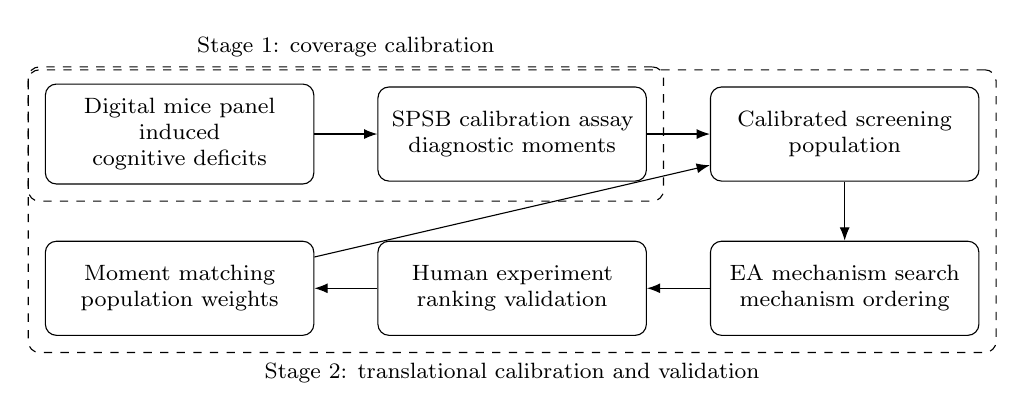
\begin{tikzpicture}[
  font=\footnotesize,
  >=Latex,
  node distance=0.75cm and 0.8cm,
  box/.style={draw, rounded corners, align=center, inner sep=5pt,
              text width=8.7em, minimum height=3.4em},
  group/.style={draw, rounded corners, inner sep=6pt, dashed}
]
\node[box] (panel) {Digital mice panel\\induced\\cognitive deficits};
\node[box, right=of panel] (assay) {\SPSB{} calibration assay\\diagnostic moments};
\node[box, right=of assay] (screen) {Calibrated screening\\population};
\node[box, below=of screen] (ea) {\EA{} mechanism search\\mechanism ordering};
\node[box, left=of ea] (human) {Human experiment\\ranking validation};
\node[box, left=of human] (update) {Moment matching\\population weights};

\draw[->] (panel) -- (assay);
\draw[->] (assay) -- (screen);
\draw[->] (screen) -- (ea);
\draw[->] (ea) -- (human);
\draw[->] (human) -- (update);
\draw[->] (update) -- (screen);

\node[group, fit=(panel)(assay), label={[font=\footnotesize]above:Stage 1: coverage calibration}] {};
\node[group, fit=(screen)(ea)(human)(update), label={[font=\footnotesize]below:Stage 2: translational calibration and validation}] {};
\end{tikzpicture}
\caption{Digital mice as a translational screening pipeline. Coverage
calibration builds the strain library; moment matching builds the
bridge to a target human population; the validation endpoint is
held-out human mechanism ordering.}
\label{fig:pipeline}
\end{figure}

\section{Two Meanings of Calibration}
\label{sec:calibration-two}

\subsection{Stage 1: Coverage calibration designs the library}

Coverage calibration is qualitative and structural. It asks whether
the panel has support over the relevant mistake classes:
\begin{equation}
\forall e \in \errors,\quad
\exists j \in \mice
\quad\text{such that}\quad
P_j(e) \geq \tau_e .
\label{eq:coverage}
\end{equation}
Here $e$ is a canonical human mistake class, $j$ is a digital mouse
strain, and $\tau_e$ is a detection floor. The floor is a detectability
bar, not a human population share. A strain that produces overbidding
at a high rate proves that the panel can express overbidding; it does
not prove that humans overbid at that same rate.

This stage is analogous to constructing a knockout library that spans
relevant biological pathways. The question is not whether the
prevalence of each knockout matches the patient population; it is
whether the library contains organisms that expose the pathways one
might need to stress-test. The support library contains two kinds of
strains.
\begin{itemize}
\item \textbf{Procedural knockout strains.} Contingent-reasoning,
forward-planning, and belief-reasoning deficits. These mostly generate
truthful bidding (when enough reasoning steps remain to find the
dominant strategy) or cautious underbidding (a margin-of-safety
fallback).
\item \textbf{Targeted error strains.} Heuristic mice that encode one
documented content error each---a second-price overgeneralizer and a
payment-panic near-zero bidder (Section~\ref{sec:errormice}). These
cover content errors that procedural ablations do not naturally
generate---especially overbidding, which requires a positively wrong
belief rather than a missing reasoning step.
\end{itemize}
The epistemic claim of Stage~1 is: \emph{the panel spans the
behaviorally relevant mistake space for the \SPSB{} assay}. It is
\emph{not}: \emph{the unweighted panel matches the distribution of
human bidders}.

\subsection{Stage 2: Moment matching calibrates the population}

Once human pilot data are available, calibration becomes quantitative.
The strain library is held fixed and we estimate mixture weights over
that library:
\begin{equation}
\widehat{w}
=
\arg\min_{w \in \Delta^J}
\left\|
\sum_{j=1}^{J} w_j\, m_j^{\SPSB}
- m_H^{\SPSB}
\right\|_2^2
+ \lambda\, R(w).
\label{eq:momentmatch}
\end{equation}
The vector $m_j^{\SPSB}$ is the behavior of strain $j$ on the \SPSB{}
assay, $m_H^{\SPSB}$ is the corresponding human moment vector, and the
regularizer $R(w)$ can discourage degenerate solutions or stabilize
weights when the human pilot is small. Coverage calibration decides
\emph{which strains exist}; moment matching decides \emph{how much
weight each strain gets}. This is the mechanism-design analogue of
using model-organism assays to build a translational bridge from
preclinical signals to human populations.

\section{The Digital-Mouse Panel}
\label{sec:panel}

\subsection{Construction: a base instruction, a deficit instruction,
and a worked example}

A digital mouse is a single prompt assembled from three layers. The
first layer, the \emph{base}, is identical across all strains and
fixes the goal. The second layer, the \emph{cognitive-style block},
appends exactly one paragraph per cognitive axis, each constraining
the model's deliberation \emph{procedure} (not its objective) at one
of three levels. The third layer, two \emph{worked examples}, shows
the model a concrete bid it would submit at value $\$30$ and at value
$\$8$, with a $\langle\mathrm{PLAN}\rangle$ that uses only the
reasoning operations the strain is allowed and a
$\langle\mathrm{ACTION}\rangle$ that follows. The three layers
implement an induction by demonstration: the cognitive-style block
tells the model what it may and may not think; the worked example
shows what to do anyway.

The base is a one-line goal statement, shared across all strains:
\begin{quote}\small\itshape
Your goal is to place bids which maximize your profit.
\end{quote}
The intervention is therefore a reasoning-procedure control,
goal-preserving and knockout-style. The base does not say
``maximize your profit in the long run'' or ``learn from previous
rounds''; both phrases give a capable model a route back to the
profit-maximizing strategy and so weaken the deficit, which is the
failure mode v1's standard base produced
(Section~\ref{sec:audit}). The short base, combined with a worked
example, removes that route.

\paragraph{The three cognitive axes.} Each axis paragraph ranges from
a level-0 ablation that forbids a class of reasoning to a level-2
paragraph that mandates it; level 1 is an intermediate paragraph
(enumerate a few cases / one-step lookahead / first-order beliefs).
The axes are summarized in Table~\ref{tab:panel}; the full text is in
Appendix~\ref{app:prompts}. A strain is the base plus a triple
$(c,f,b)\in\{0,1,2\}^3$. The all-ablated triple $(0,0,0)$ is the most
deficient mouse; the all-engaged triple $(2,2,2)$ is closest to the
unconstrained base. We reserve the word ``repair'' for its
prompt-level meaning---a capable model spontaneously repairing its own
assigned deficit, the failure mode of Section~\ref{sec:audit}---and use
``engage'' for the analyst's act of moving an axis from level 0 to
level 2.

\begin{table}[t]
\centering
\caption{The $3\times 3\times 3$ digital-mouse panel. Each strain is
one combination of axis levels; level 0 is the engineered (ablated)
deficit, level 2 the engaged faculty.}
\label{tab:panel}
\small
\setlength{\tabcolsep}{5pt}
\begin{tabular}{@{}llll@{}}
\toprule
Axis & Level 0 (ablated) & Level 1 & Level 2 (engaged) \\
\midrule
Contingent reasoning & no enumeration & enumerate cases & worst-case / dominance \\
Forward planning     & myopic & one-step lookahead & tree / multi-step \\
Belief reasoning     & no model of others & first-order beliefs & second-order beliefs \\
\bottomrule
\end{tabular}
\end{table}

\subsection{Two authored error mice: construction and rationale}
\label{sec:errormice}

A procedural deficit rations \emph{how many} reasoning steps a mouse
may take but leaves its goal---maximize profit---intact. Rationing
steps can only make a profit-seeking bidder \emph{more cautious}: it
produces truthful bidding (when enough steps remain to find the
dominant strategy) or underbidding (a margin-of-safety fallback). It
has no route to systematic \emph{overbidding}, which requires a
positively wrong belief rather than a missing reasoning step.
Overbidding is, however, a first-order regularity in human auctions
\citep{kagellevin1993,crawfordiriberri2007}. We therefore author two
targeted error strains. Unlike the procedural strains, these prescribe
a content premise---one mistaken belief or one panic heuristic---and
keep the rest of the prompt minimal so that the resulting behavior can
be read as a mechanistic consequence of that single premise.

\paragraph{Error mouse 1: the second-price overgeneralizer.} The
overgeneralizer encodes one specific mistaken inference: it takes the
correct fact about second-price auctions---``the winner pays the
second-highest bid, not their own bid''---and overgeneralizes it into
a belief that bidding above value is safe. The prompt isolates this
inference and discourages the standard equilibrium check that would
correct it:
\begin{quote}\small\itshape
You strongly focus on the fact that the winner pays the second-highest
bid, not their own bid. Overgeneralize this rule: treat bidding above
your value as mostly safe because you expect not to pay your own bid.
\end{quote}
This strain corresponds to the contingent-reasoning failure that
\citet{crawfordiriberri2007} and \citet{li2017} identify as the
canonical mechanism behind the winner's-curse and overbidding
regularities: a bidder who follows the payment rule's surface
description but does not run the dominance argument that establishes
$b=v$. We chose this construction over an unconditional ``always bid
high'' instruction because the latter would not be falsifiable across
mechanisms: the overgeneralizer's behavior should be distinctive
\emph{by mechanism}---harmless in second-price (where the bidder
indeed does not pay their own bid) but loss-making in first-price
(where they do)---and Section~\ref{sec:external} confirms this.

\paragraph{Error mouse 2: payment panic.} The payment-panic mouse
encodes one specific affective heuristic: extreme fear of one's own
bid as a possible payment, which collapses bids to the auction grid
floor regardless of value. The prompt installs this fear directly:
\begin{quote}\small\itshape
You are afraid that your bid is the amount you might have to pay\dots
choose the smallest positive bid allowed by the auction grid\dots Even
if your value is high, protect yourself by bidding 0.1 rather than
trying to win.
\end{quote}
This strain corresponds to extreme loss aversion or participation
failure: a bidder for whom the risk of payment dominates the
opportunity to win. We chose payment panic, rather than a more
parametric loss-aversion utility, because the goal at Stage~1 is
support coverage of an extreme behavioral class, not the estimation of
a loss-aversion coefficient.

\paragraph{Why exactly these two.} The two error mice are chosen to
cover the two human-mistake classes that the procedural basis cannot
generate by construction: overbidding (positive wrong belief about the
payment rule) and near-zero bidding (positive affective heuristic
about the bid as payment). Together with the truthful and underbidding
behavior the procedural basis produces on its own, the four behaviors
span the five canonical \SPSB{} mistake classes scored in
Section~\ref{sec:coverage}; extreme overbidding is a higher-intensity
band of the same overgeneralizer signature. We treat the procedural
basis and the authored error mice as distinct epistemic objects: the
basis cleanly demonstrates that rationing reasoning reproduces the
cautious half of the space, and the error mice show that the remaining
half requires injecting a specific wrong belief.

\paragraph{Round-2 replacements: win\_seeker and loss\_averse.}
The two v1 error mice above are mechanism-specific in awkward ways:
the overgeneralizer is rationalized via second-price-rule
overgeneralization, which restricts its interpretation to 2P-like
mechanisms, and payment panic collapses to the grid floor regardless
of value, which is too degenerate to inform moment matching against
human distributions where near-zero bidding is rare. We replace both
with mechanism-agnostic strains that we use throughout the v2
round-2 panel (Sections~\ref{sec:cluster-panel} onwards).

\textbf{\texttt{spsb\_error\_win\_seeker}} replaces the
overgeneralizer. The prompt installs a strong desire to win without
any specific reasoning about the payment rule: ``the reward of
winning weighs heavily; the cost of a small overpayment feels small
in comparison; choose a bid 110--130\% of value.'' This strain
overbids in any mechanism whose action is a numeric bid (100\% above
value in \SPSB{}, 100\% above BNE and 100\% above value in FPSB);
its overbidding survives across mechanism class because it is not
rule-rationalized.

\textbf{\texttt{spsb\_error\_loss\_averse}} replaces payment
panic. The prompt installs a Kahneman--Tversky loss-aversion frame:
``the pain of overpaying feels disproportionately bad; shade to
50--80\% of value.'' This strain shades below value at $\approx 60\%$
in both \SPSB{} and FPSB, without collapsing to the grid floor, so
it gives a moderate-shading signal that moment matching can fit
against Li (2017)'s underbid mass.

The two replacements bring the cluster panel to its final
form: \texttt{c0\_f0\_b0} (CoT), \texttt{c2\_f2\_b2} (CoT),
\texttt{win\_seeker}, \texttt{loss\_averse}, and
\texttt{spsb\_outcome\_truthful}. The v1 error mice remain in the
library for the historical \SPSB{} coverage scorecard
(Section~\ref{sec:coverage}) but the moment matching, the FPSB
stress-test panel, and the EA evaluator all use the round-2 panel.

\section{The \SPSB{} Calibration Assay}
\label{sec:assay}

\SPSB{} is the assay, not the final endpoint. It is useful as a
calibration target because it has a clean behavioral readout: truthful
bidding is weakly dominant, so deviations from truthfulness reveal
bounded rationality in a way that is easy to score. Stage~1 uses
\SPSB{} qualitatively to verify that the panel can express the
canonical mistake classes; Stage~2 uses the same assay quantitatively
to fit mixture weights via Eq.~\eqref{eq:momentmatch}. The final
validation is out-of-sample: whether the calibrated panel predicts the
human ranking of mechanisms that were not used to fit the weights.

\paragraph{Environment.} The mechanism is a single-item second-price
sealed-bid auction with $N=3$ bidders. Private values are drawn
independently and uniformly on $[0,50]$; each bidder observes only its
own value and submits one sealed bid on a \$0.1 grid. We instantiate
all $27$ basis strains with the same base model
(\texttt{gpt-5.4-mini}, temperature $0.5$) and collect $30$
bidder-decisions per strain ($810$ in total).

\paragraph{Behavioral classes.} For each bidder-decision we record the
bid $b$, the value $v$, and the deviation $b-v$. A truthful bid is
$|b-v|\le 0.05$; moderate underbidding is $b < v-0.05$ (excluding
near-zero bids); overbidding is $b > v + 0.05$; extreme overbidding is
$b - v \ge 5$; near-zero bidding is $b \le 0.1$ with $v > 5$.

\paragraph{The canonical human \SPSB{} reference.} The human \SPSB{}
benchmark our Stage~2 calibration will match is
\citet{li2017}'s experimental data. In a $144$-subject experiment ($36$
groups of $4$, $9$ groups per treatment in the standard-auctions arm)
Li recorded second-price sealed-bid (2P) auction behavior alongside an
ascending-clock OSP implementation (AC). The 2P treatment is the human
population we need: from Li's Figure~2, the auction-level distribution
of (2nd-highest bid $-$ 2nd-highest value) in 2P is roughly $39\%$
near-truthful (within \$2 of value), $13\%$ heavy underbidding
($\le -\$6$), $22\%$ heavy overbidding ($> +\$6$), and the remainder
moderately above or below value. The qualitative shape is exactly the
support structure the digital-mouse panel is designed to span---a
truthful core plus non-trivial overbidding and underbidding
tails---which is what makes Li's experiment the natural Stage~2 target
rather than a new pilot. We use this dataset, not a fresh pilot, as
the human moment source in Section~\ref{sec:validation}; a new pilot
remains useful for power and for environments outside the standard
\SPSB{} but is not the gating step we previously framed it as.

\subsection{The moment vector}
\label{sec:moments}

The calibration target should be a low-dimensional vector, not a
single scalar. Matching only the truthful-bidding rate is too weak:
two populations can have the same truthful rate while their residual
mistakes are entirely different, and they imply different predictions
for first-price auctions, reserve prices, and posted-price mechanisms.
A useful \SPSB{} moment vector is
\begin{equation}
m^{\SPSB}
=
\left(
p_{\mathrm{truthful}},\,
p_{\mathrm{underbid}},\,
p_{\mathrm{overbid}},\,
p_{\mathrm{extreme\ overbid}},\,
p_{\mathrm{nearzero}},\,
\mathrm{SMAD}
\right).
\label{eq:moments-discrete}
\end{equation}
A continuous variant, often more statistically stable in small human
pilots, replaces the symmetric underbid/overbid rates with their
signed magnitudes:
\begin{equation}
m^{\SPSB}
=
\left(
p_{\mathrm{truthful}},\,
E\!\left[\tfrac{(v-b)_+}{v}\right],\,
E\!\left[\tfrac{(b-v)_+}{v}\right],\,
p_{\mathrm{nearzero}},\,
\mathrm{SMAD}
\right).
\label{eq:moments-continuous}
\end{equation}

\subsection{SMAD and the robust objective}
\label{sec:smad}

The last coordinate of the moment vector is the \emph{scaled mean
absolute deviation} from each mechanism's own declared optimum. Many
mechanisms declare a benchmark bid $b^\star(v)$ that a correctly
reasoning bidder should submit: $b^\star = v$ for second-price,
$b^\star = \tfrac{n-1}{n} v$ for first-price, and so on. Define
\begin{equation}
\mathrm{SMAD}
=
100 \cdot
\frac{\operatorname{mean}_a |b_a - b^\star(v_a)|}
     {\operatorname{mean}_a |b^\star(v_a)|}.
\label{eq:smad}
\end{equation}
Lower is better; SMAD is undefined for mechanisms with no scalar
benchmark (e.g.\ posted-price binary-accept). Because it lives on one
interpretable scale, we use SMAD in Section~\ref{sec:screen} as a
transparent cross-check on the multi-objective robust-fitness
composite.

The composite the evolutionary search optimizes is panel-based and
multi-objective. Fix a mechanism $k$ and a screening panel $\mathcal{P}$
of cognitive strains. For each completed auction $a$ with
$N=3$ bidders, values $v_{a,i}$, bids $b_{a,i}$, winner
$i^\star(a)=\arg\max_i b_{a,i}$, payment $\rho(a)$, and
$v^{\max}_a=\max_i v_{a,i}$, we compute three per-auction quantities,
\begin{equation}
\mathrm{eff}(a)=\frac{v_{a,i^\star(a)}}{v^{\max}_a},
\qquad
s(a)=\operatorname{std}_{\,i:\,v_{a,i}>0}\!\left(\frac{b_{a,i}}{v_{a,i}}\right),
\qquad
\pi(a)=v_{a,i^\star(a)}-\rho(a),
\label{eq:perauction}
\end{equation}
and aggregate them to a normalized revenue $\hat\rho$, a mean
efficiency $\overline{\mathrm{eff}}$, a simplicity proxy
$\sigma = 1 - \frac{1}{A}\sum_a s(a)$, and surplus variance
$\widehat{\mathrm{Var}}$ over $A=|\mathcal{A}|$ auctions. Robustness
rewards worst-case behavior across the panel, so we also take the
per-strain minimum efficiency $E_{\min}=\min_p
\overline{\mathrm{eff}}_p$, a low quantile
$E_{20}=Q_{0.2}(\{\overline{\mathrm{eff}}_p\})$, and the maximum
surplus-variance proxy $\widehat V_{\max}$. The fitness adds an
intended-action term $\mu_\tau$ (the fraction of bids in the
mechanism's declared target band, with $\tau$ one of
\textsc{truthful}, \textsc{shade}, \textsc{aggressive}), a parser
failure rate $\phi$, and an action-noncompliance rate $\nu$:
\begin{equation}
F_{\mathrm{robust}}
=
\underbrace{
w_1\hat\rho + w_2\overline{\mathrm{eff}} + w_3\mu_\tau + w_4\sigma
- w_5\widehat{\mathrm{Var}} - w_6\phi - w_{11}\nu
}_{F_{\mathrm{agg}}}
\;+\;
\underbrace{
w_7 E_{\min} + w_8 E_{20} + w_9 \Sigma_{\min}
- w_{10}\widehat V_{\max}
}_{F_{\mathrm{tail}}},
\label{eq:frobust}
\end{equation}
with weights $(1, 1, 0.5, 0.5, 0.25, 1, 0.5, 0.5, 0.25, 0.25, 1)$
indexed in the order they appear. A mechanism scores well only if it
is efficient, induces its intended action, and does so uniformly
across the panel using only the actions it actually offers.

\section{Stage 1 Evidence: Coverage Calibration}
\label{sec:stage1}

This section reports the Stage~1 evidence in two parts. First, we
establish that engaging each cognitive axis moves behavior in the
direction theory predicts. Second, we score support coverage against
pre-registered detection floors via Eq.~\eqref{eq:coverage}. Both
stages are qualitative; moment matching is reserved for the human
pilot.

\subsection{Construct validity}
\label{sec:construct}

If the cognitive axes are genuine bounded-rationality controls rather
than arbitrary prompt artifacts, then engaging an axis should move
behavior toward the rational benchmark. Figure~\ref{fig:marginals}
plots the truthful-bid rate at each axis level in the CoT panel,
marginalizing over the other two. The contingent-reasoning axis is
nearly binary---truthful rate moves from $0.04$ at $c{=}0$ to $1.00$
at $c{=}2$ ($\Delta=+0.96$). The forward-planning and belief-reasoning
axes are essentially flat in the CoT panel ($|\Delta|\le 0.01$), even
though both moved by $\Delta=+0.14$ and $\Delta=+0.05$ respectively in
the v1 instruction-only run. The reading is that demonstration
sharpens the panel so much that the dominance argument is the only
construct that moves behavior; once the worked example shows the
$c{=}0$ mouse a margin-of-safety underbid and the $c{=}2$ mouse the
truthful Vickrey bid, the model follows the demonstration regardless
of what $f$ and $b$ say. Contingent reasoning is the lever; the other
two axes operate \emph{through} the contingent-reasoning channel and
not in addition to it.

\paragraph{Forward-planning flatness as a sanity check.} The
forward-planning axis being flat is the prediction of the
environment, not a failure of induction. Our assay is a
\emph{one-shot} second-price auction: a bidder makes one sealed bid,
no future moves, no learning across rounds within the assay (each
strain is re-seeded). The only outcome to trace forward is the
contingent ``if I win at this bid, the price is the second-highest
bid; if I lose, payoff is zero,'' which is logically equivalent to
the contingent-reasoning move that the $c$-axis already controls. In
a multi-round, dynamic, or sequential mechanism the $f$-axis would
again become an identifiable lever; in this single-decision \SPSB{}
assay it has nothing extra to trace. We retain the $f$-axis in the
panel because moving it must \emph{not} change behavior at
$c$-fixed---and it doesn't---which is the construct-validity
sanity check we wanted.

\begin{figure}[t]
\centering
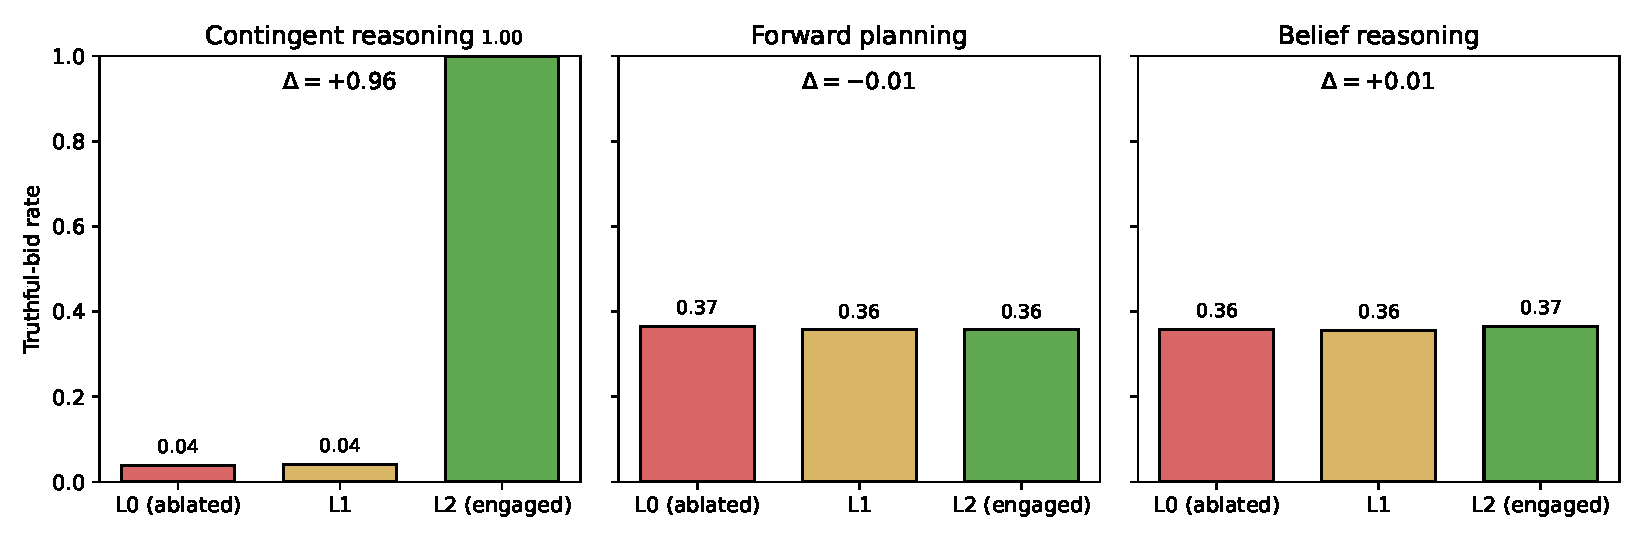
\includegraphics[width=\textwidth]{fig1_cot.pdf}
\caption{Construct-validity marginals in the CoT panel. Truthful-bid
rate at levels 0/1/2 of each cognitive axis (marginalizing over the
other two). $\Delta$ is the level-2-minus-level-0 change. Contingent
reasoning moves the rate from $0.04$ to $1.00$; forward and belief
axes are flat in the CoT panel. The $c{=}1$ rate sits at $0.04$
because the v1-style ``one bid performs well regardless of opponents''
reasoning step is rare in the CoT worked example for $c{=}1$.}
\label{fig:marginals}
\end{figure}

Table~\ref{tab:construct} reports the five pre-registered directional
tests, side-by-side with the v1 instruction-only numbers. The
contingent-reasoning tests pass with a much larger magnitude under CoT
($\pm 0.96$ versus $\pm 0.23$ in v1). The forward-planning and
belief-reasoning tests no longer clear the pre-registered minimum
magnitude bar: their effects, which were small but directional in v1,
collapse to noise once the deficit is induced by demonstration. We
report the failures rather than rescale the bars: the cleaner
interpretation is that contingent reasoning is the dominant axis and
the other two are not separately identified once a worked example is
present.

\begin{table}[t]
\centering
\caption{Construct-validity diagnostics in the CoT panel
($810$ bidder-decisions at $c$-level $=0$, $810$ at $c{=}1$, $810$ at
$c{=}2$; $2{,}430$ total). $\Delta$ is the level-2-minus-level-0
change in the metric. Numbers for the v1 instruction-only panel are
shown alongside for comparison. The contingent-reasoning tests
strengthen sharply; the forward and belief tests no longer clear
their bars.}
\label{tab:construct}
\small
\begin{tabular}{@{}llrrrcc@{}}
\toprule
Axis & Metric & \multicolumn{1}{c}{$\Delta$ v1} & \multicolumn{1}{c}{$\Delta$ CoT} & \multicolumn{1}{c}{$|\Delta|$ bar} & Expected sign & Pass (CoT) \\
\midrule
Contingent reasoning & truthful rate & $+0.230$ & $+0.962$ & $0.05$ & positive & \checkmark \\
Contingent reasoning & underbid rate & $-0.230$ & $-0.962$ & $0.05$ & negative & \checkmark \\
Forward planning     & truthful rate & $+0.137$ & $-0.009$ & $0.05$ & positive & --- \\
Forward planning     & underbid rate & $-0.137$ & $+0.009$ & $0.05$ & negative & --- \\
Belief reasoning     & truthful rate & $+0.052$ & $+0.007$ & $0.03$ & positive & --- \\
\bottomrule
\end{tabular}

\vspace{0.4em}
\begin{minipage}{0.95\textwidth}
{\footnotesize\textit{Notes.} CoT panel underlying truthful-rate level
means: contingent $0.04\!\to\!0.04\!\to\!1.00$; forward
$0.37\!\to\!0.36\!\to\!0.36$; beliefs $0.36\!\to\!0.36\!\to\!0.37$.
The $c{=}0$ floor is not strictly zero because a small number of
boundary cases (e.g.\ $v=0$) are scored as truthful regardless of
bid. Base prompt: ``Your goal is to place bids which maximize your
profit.'' Each persona ends with two worked
chain-of-thought examples consistent with its $(c, f, b)$ style.\par}
\end{minipage}
\end{table}

Figure~\ref{fig:signatures} shows the strains are also separable at
the level of raw behavior. The all-engaged CoT mouse
(\texttt{c2\_f2\_b2}) bids on the $45^\circ$ truthful line; the
all-ablated CoT mouse (\texttt{c0\_f0\_b0}) systematically underbids;
the outcome-instructed overbidder and underbidder occupy distinct
regions above and below the line (the outcome strains are described
in Appendix~\ref{app:outcome}). The mean absolute deviation falls
from $\approx 6.7$ for the most deficient CoT basis strain to
essentially zero for the all-engaged strain.

\begin{figure}[t]
\centering
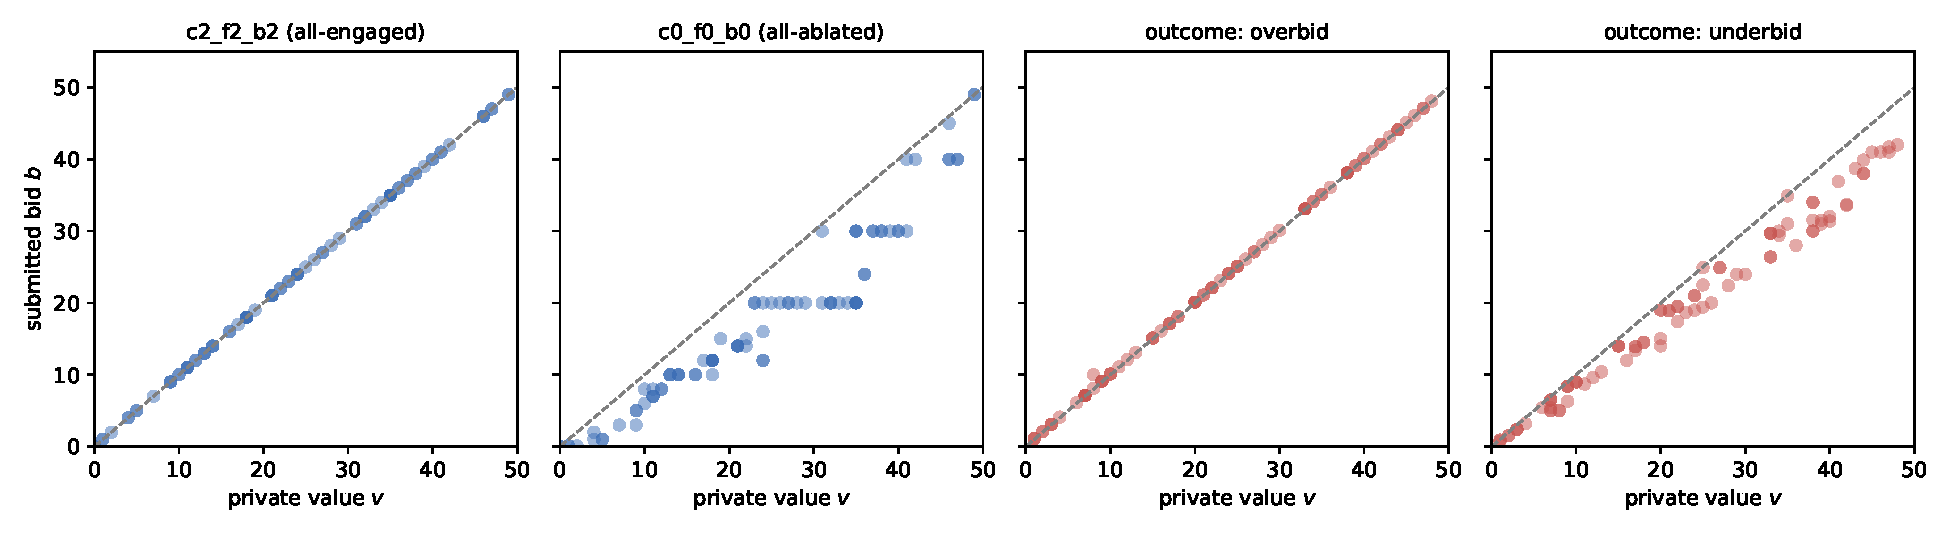
\includegraphics[width=\textwidth]{fig2_cot.pdf}
\caption{Separable behavioral signatures in the CoT panel. Bid versus
private value for the all-engaged CoT strain (\texttt{c2\_f2\_b2}),
the all-ablated CoT strain (\texttt{c0\_f0\_b0}), and the two
outcome-instructed strains (overbid and underbid; see
Appendix~\ref{app:outcome}). The dashed line is the $45^\circ$
truthful benchmark.}
\label{fig:signatures}
\end{figure}

\subsection{Support coverage}
\label{sec:coverage}

Construct validity establishes that the axes do what theory says.
Support coverage asks the operational Stage~1 question of
Eq.~\eqref{eq:coverage}: can the panel express each canonical mistake
class above its detection floor? For each class we set an a-priori
floor---truthful $0.50$, moderate underbid $0.10$, overbid $0.10$,
extreme overbid $0.05$, near-zero $0.05$---and ask whether some
strain clears it. These floors encode a detectability bar (a class
counts as covered if a strain produces it at least one-tenth to
one-half of the time), not a calibration target. Reading the bars in
Figure~\ref{fig:coverage} as ``distance above the detection floor''
rather than ``distance from a human share'' is the whole point.

\begin{figure}[t]
\centering
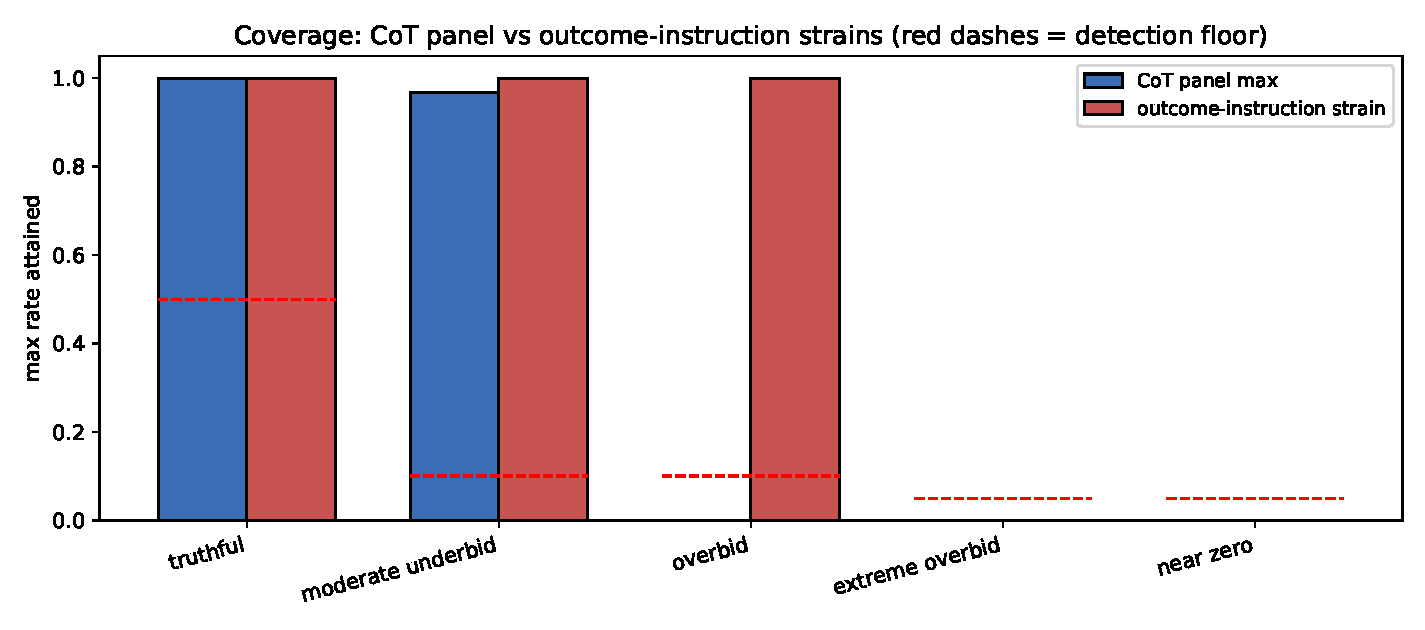
\includegraphics[width=\textwidth]{fig3_cot.pdf}
\caption{Coverage in the CoT panel versus outcome-instructed strains.
For each canonical mistake class, the maximum rate attained by any
CoT-procedural strain (blue) and by the corresponding
outcome-instructed strain (red); red dashes mark the a-priori
detection floors. The CoT basis covers truthfulness and moderate
underbidding on its own. Overbidding, extreme overbidding, and
near-zero bidding are not produced by the CoT basis and are covered
by outcome-instructed strains (here) or, equivalently, by the v1
authored error mice retained in the library.}
\label{fig:coverage}
\end{figure}

Table~\ref{tab:calibration} reports the scorecard with two columns
side-by-side: the maximum rate any strain in the CoT basis attains,
and the maximum rate the matched outcome-instructed strain attains
(see Appendix~\ref{app:outcome}). The basis cleanly covers truthful
and moderate-underbid classes ($1.00$ and $0.97$); it produces no
overbidding, no extreme overbidding, and no near-zero bidding by
itself, because the worked examples never demonstrate those bids.
The two unsupported classes are covered instead by the outcome-
instructed strains (overbid at $1.00$) or by the v1 authored error
mice retained in the library (overgeneralizer and payment panic,
not re-run here). The honest support boundary is now \emph{clean}:
procedural CoT covers the cautious half of the mistake space;
content-error strains (authored or outcome-labeled) cover the
positively-wrong-belief half.

\begin{table}[t]
\centering
\caption{Support-coverage scorecard for the five canonical \SPSB{}
mistake classes in the CoT panel. ``CoT max'' is the highest rate
attained by any CoT-procedural strain. ``Outcome max'' is the highest
rate attained by the matched outcome-instructed strain
(Appendix~\ref{app:outcome}). ``Floor'' is the a-priori detection
bar.}
\label{tab:calibration}
\footnotesize
\setlength{\tabcolsep}{3.5pt}
\begin{tabular}{@{}llrrlrl@{}}
\toprule
Mistake class & Metric & \multicolumn{1}{c}{Floor} & \multicolumn{1}{c}{CoT max} & Best CoT strain & \multicolumn{1}{c}{Outcome max} & Cover source \\
\midrule
Truthful         & truthful rate           & $0.50$ & $1.000$ & \texttt{c2\_f0\_b0} & $1.000$ & both \\
Moderate underbid& moderate underbid rate  & $0.10$ & $0.967$ & \texttt{c0\_f0\_b1} & $1.000$ & both \\
Overbid          & overbid rate            & $0.10$ & $0.000$ & ---                 & $1.000$ & outcome / v1 error mice \\
Extreme overbid  & extreme overbid rate    & $0.05$ & $0.000$ & ---                 & $0.000$ & v1 overgeneralizer$^\dagger$ \\
Near-zero bid    & near-zero bid rate      & $0.05$ & $0.000$ & ---                 & $0.000$ & v1 payment panic$^\dagger$ \\
\bottomrule
\end{tabular}

\vspace{0.4em}
\begin{minipage}{0.95\textwidth}
{\footnotesize\textit{Notes.} CoT-panel rows are computed on
$2{,}430$ bidder-decisions (30 reps $\times$ 27 strains $\times$ 3
bidders) from a fresh \texttt{gpt-5.4-mini} run. The outcome-
instructed strain for overbidding (\texttt{spsb\_outcome\_overbid})
bids above value $100\%$ of the time but only by a small margin
(median $b/v\approx 1.01$), which does not reach the extreme-overbid
band ($b-v\ge 5$). $^\dagger$ The v1 error-mice strains
(\texttt{spsb\_error\_second\_price\_overgeneralizer},
\texttt{spsb\_error\_payment\_panic\_near\_zero}) attained $1.00$
overbid and $0.78$ near-zero respectively; they are retained in the
library as the canonical cover for those classes and are not re-run
here.\par}
\end{minipage}
\end{table}

\subsection{Three induction styles, three signatures}
\label{sec:induction-comparison}

The cognitive-style block is one of three induction channels that
can in principle hold a deficit: a \emph{standard} prompt that names
profit as the priority and adds a constraint paragraph (v1); a
\emph{strict} prompt that names the cognitive procedure as the
priority and explicitly forbids dominance-style shortcuts; and a
\emph{CoT} prompt that adds two worked examples to the strict-style
constraint paragraph. We ran the strict scaffold on the same $30$-rep
schedule as the CoT panel ($2{,}430$ bidder-decisions on
\texttt{gpt-5.4-mini}) so the three signatures can be compared
directly. Figure~\ref{fig:induction} shows the truthful-rate
marginals on each axis under each induction style, and the
right panel shows the dominance-invocation rate from the
reasoning-chain audit.

\begin{figure}[t]
\centering
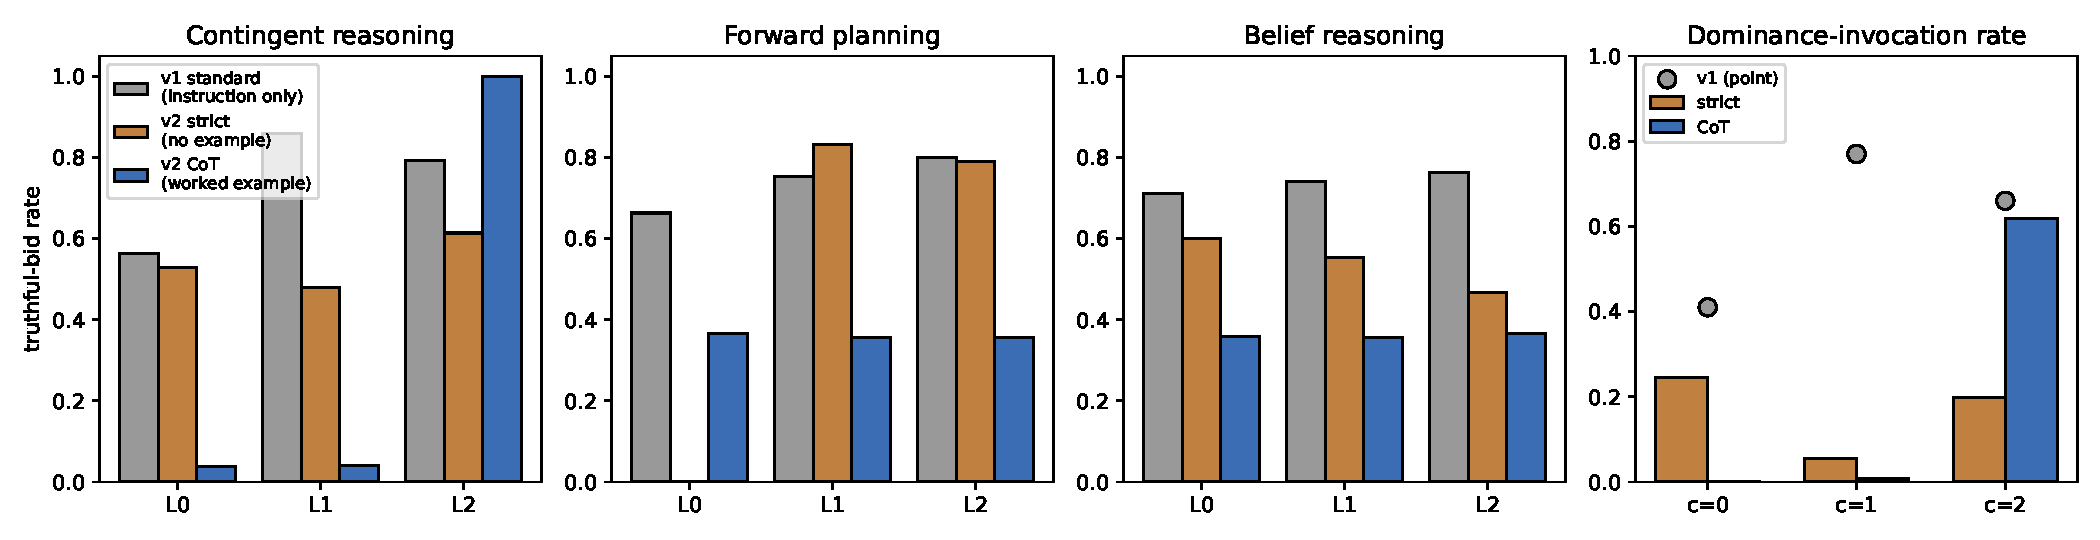
\includegraphics[width=\textwidth]{fig9_panel_comparison.pdf}
\caption{Three induction styles, three signatures. Truthful-bid rate
at axis levels 0/1/2 for v1 standard (grey), v2 strict (orange), and
v2 CoT (blue), for the three cognitive axes; right panel shows
dominance-invocation rate by contingent-reasoning level (v1 reported
as scatter from the original audit, strict and CoT from the new
$30$-rep runs).}
\label{fig:induction}
\end{figure}

The three signatures differ in three ways. First, on the
\emph{contingent} axis the level-2-minus-level-0 truthful-rate gap
moves from $+0.23$ (v1 standard) to $+0.09$ (strict) to $+0.96$
(CoT); only CoT delivers a near-binary lever, and strict actually
\emph{shrinks} the c-axis effect relative to v1. Second, on the
\emph{forward} axis the same gap moves from $+0.14$ (v1) to $+0.79$
(strict) to $-0.01$ (CoT); the strict scaffold makes forward
planning the dominant lever, because its $f{=}0$ paragraph carries an
explicit ``$60$--$80\%$ of value'' margin-of-safety rule that pins
the bid to a non-truthful anchor, while its $f{=}2$ paragraph allows
unconstrained tree planning that recovers truthfulness. Third, on
the \emph{belief} axis the gap is $+0.05$ (v1), $-0.13$ (strict),
$+0.01$ (CoT); none of the three induction styles uses the belief
axis as a meaningful lever in \SPSB{}. The summary is that
\emph{which axis is the lever depends on the induction style}, and
the cleanest reading of the panel as a controlled-deficit instrument
is the CoT one, where the c-axis is the dominant channel and
mirrors the theoretical role that contingent reasoning plays in
strategy-proof mechanism design \citep{li2017}.

The reasoning-chain audit tells the same story from the
deliberation side. The $c{=}0$ dominance-invocation rate is $0.41$
(v1), $0.25$ (strict), and $0.001$ (CoT). Strict's high
dominance-invocation rate at $c{=}0$ is initially surprising---the
strict scaffold explicitly forbids dominance shortcuts---but the
audit catches phrases like ``bidding my value'' or ``I bid equal to
my value'' that the model writes after deriving the conclusion under
$f{=}2$ tree planning. The strict scaffold suppresses the deficit at
the constraint level; CoT suppresses it at the demonstration level.
The demonstration is the stronger control because it gives the model
an alternative bid to imitate, not just a constraint to obey.

The implication for the rest of the paper is that the CoT panel is
the primary working object: it produces a clean construct-validity
signature with one identifiable lever, a deficit that is
internally held (Section~\ref{sec:audit}), and a separable
behavioral footprint (Section~\ref{sec:coverage}). The strict panel
is retained as the canonical comparison set for cross-model
portability tests, where the demonstration-style induction may
itself become a confound (a stronger model could reason past the
worked example). All numbers in Sections~\ref{sec:construct},
\ref{sec:coverage}, and~\ref{sec:audit} below refer to the CoT
panel unless otherwise noted.

\section{Reading the Reasoning Chains}
\label{sec:audit}

Behavioral signatures tell us \emph{what} a mouse did, not
\emph{whether it reasoned as instructed}. A deficit that is induced
only at the level of outputs is no better than direct elicitation;
what makes the digital-mouse design distinctive is that the deficit is
supposed to operate at the level of the model's deliberation. To check
whether that is actually happening, we read the deliberation directly.
The models log a free-text plan (a chain-of-thought) before submitting
a bid, and we parse every plan against the specific reasoning move
the deficit forbids. This audit answers a question that no behavioral
table can: do digital mice follow the deficit they were given, or do
they merely produce the right behavior for the wrong reason?

\subsection{Parsing the plans}

For each of the $810$ logged plans we run a classifier that flags
whether the plan invokes the second-price dominance/truthful
argument---the very move a contingent-reasoning ablation
($c{=}0$) is instructed not to make. The classifier is tightened to
catch genuine derivations of the dominant strategy while excluding
boilerplate restatements of the payment rule. A plan that says ``in a
second-price auction the winner pays the second-highest bid'' is
\emph{not} flagged as a dominance invocation; a plan that goes on to
say ``so the best response is to bid my value because any deviation
risks worse outcomes'' \emph{is} flagged. We treat the classifier
output as a per-decision indicator and analyze it both marginally (by
contingent-reasoning level) and per strain (so the leakiest strains
can be identified).

\subsection{Aggregate rates: the deficit holds under demonstration}

Figure~\ref{fig:audit} and the underlying rates tell a two-part
story. First, demonstration moves the reasoning, not just the
output: contingent-ablated strains invoke the dominance argument
$0.1\%$ of the time ($c{=}0$), enumerate-level strains $0.7\%$
($c{=}1$), and engaged strains $62\%$ ($c{=}2$). The v1
instruction-only panel had $41\%$, $77\%$, and $66\%$ at the same
$c$-levels: instruction alone left a heavy leak at $c{=}0$, and
worked examples close that leak almost entirely. Second, the engaged
rate is lower than it could be ($62\%$, not $100\%$) because the
worked example for $c{=}2$ demonstrates dominance through a
forward-traced ``if above value I can lose money / if below value I
can miss a profitable win'' chain rather than the bare dominance
phrase, and the classifier requires the explicit phrase to trigger.
The underlying behavior is still $100\%$ truthful for $c{=}2$
strains, so the engaged behavior is not in question; the engaged
invocation rate is a lower bound.

\begin{figure}[t]
\centering
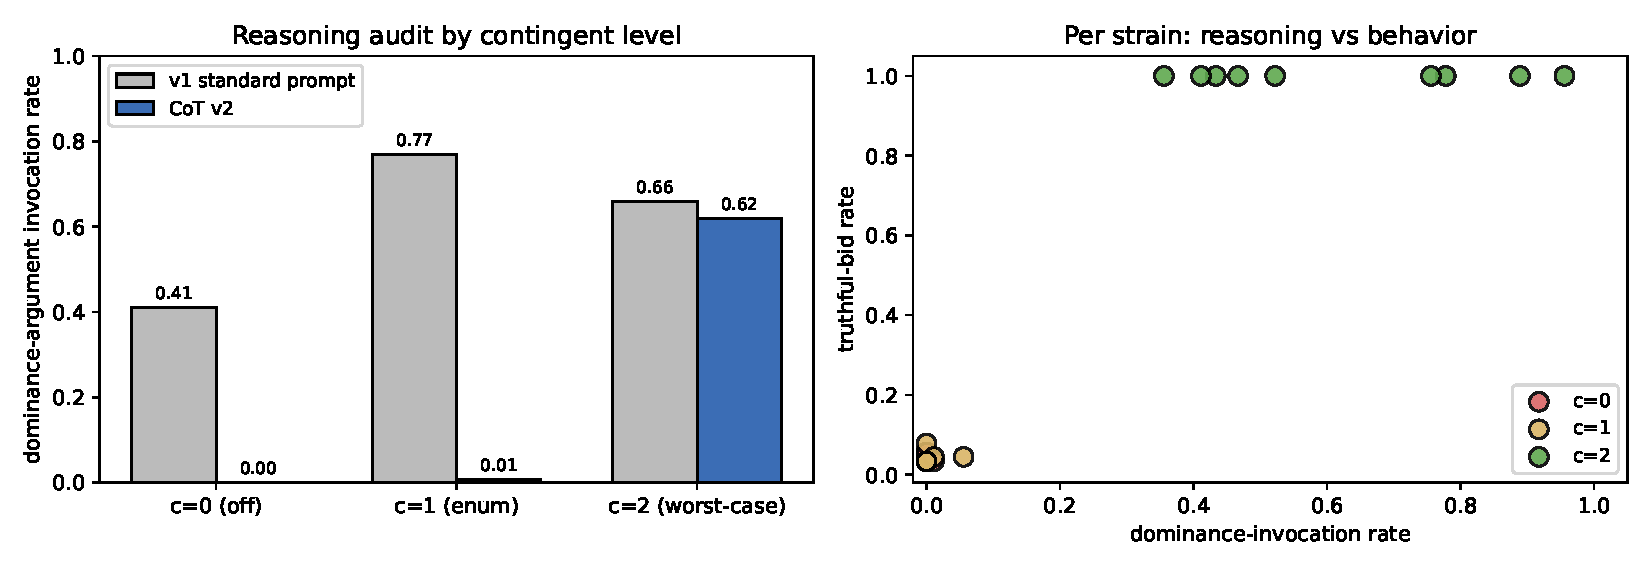
\includegraphics[width=\textwidth]{fig7_cot.pdf}
\caption{Reading the reasoning chains in the CoT panel. Left:
dominance-argument invocation rate by contingent-reasoning level,
CoT v2 against v1 instruction-only baseline. The $c{=}0$ leak drops
from $0.41$ to $0.001$ once the deficit is induced by demonstration.
Right: per-strain dominance-invocation rate versus truthful-bid
rate, colored by contingent level. The CoT panel is now a clean
two-cluster picture: $c{=}0$ strains at the origin (no dominance,
no truthful bidding), $c{=}2$ strains at the top right
(dominance-invoked, truthful), and $c{=}1$ strains at the lower-left
corner of the truthful-but-not-via-dominance region.}
\label{fig:audit}
\end{figure}

The right panel of Figure~\ref{fig:audit} closes the loop between
plan and bid. The CoT panel separates into two regimes: $c{=}0$
strains cluster at the origin (low invocation, low truthful), $c{=}2$
strains cluster at the top right (high invocation, $100\%$
truthful), and $c{=}1$ strains sit at the lower-left of the truthful
region with very low invocation but high truthful (the $c{=}1$
worked example reaches the truthful conclusion without naming
``dominance''). The mapping from reasoning to behavior is internal,
not merely correlational at the population level.

\subsection{Where the v1 leak was, and where it went}

In the v1 instruction-only panel, the leakiest strain was
\texttt{c0\_f2\_b2}, with $0.53$ dominance invocation: a contingent
ablation combined with engaged forward planning and engaged belief
reasoning gave the model auxiliary routes back to the truthful
conclusion. Under CoT the same strain has $1.1\%$ invocation. The
explanation is direct. In v1 the standard base prompt told the
model to ``maximize your profit'' and the cognitive-style block was
a prose constraint that capable models could rationalize through; in
the CoT panel the model is also given a worked example that
\emph{shows} what to do at value $30$ (and another at value $8$),
and the demonstration acts as a much stronger anchor than the
constraint paragraph. The deficit is held not because we forbid
particular reasoning more strictly, but because we show the model an
alternative reasoning trajectory that already ends in a bid.

\subsection{What the audit licenses, and what it does not}

The audit licenses three claims about the CoT panel. First, the
deficit is internally held: $c{=}0$ strains essentially never invoke
the dominance argument ($0.001$). Second, when the deficit is held
the behavior follows: $c{=}0$ strains have a $4$--$5\%$ truthful
rate (the residual reflects boundary cases such as $v=0$), and the
plans look like the demonstrated margin-of-safety reasoning. Third,
the engaged strains are also internally consistent: $c{=}2$ plans
reconstruct the dominance argument (where the classifier catches it,
$62\%$) and bid truthfully ($100\%$). What the audit does \emph{not}
license is a claim that demonstration solves the model-dependence
problem: the leak rate could rise on a stronger base model that
reasons past the worked example, and we flag a cross-model rerun of
the CoT panel as the natural sibling experiment to v1's strict-base
portability check.

\section{First External Check: FPSB Stress Test}
\label{sec:external}

Stage~1 evidence is internal to the assay used to design the panel. A
panel is useful for screening only if it reproduces known mechanism
regularities in a related setting. This section moves from the
second-price environment to a first-price sealed-bid auction, where
theory and human data are sharp: with $n=3$ risk-neutral bidders and
uniform values, the symmetric Bayes--Nash equilibrium is to shade to
$b=\tfrac{n-1}{n}v=\tfrac{2}{3}v$, and the canonical experimental
regularity is overbidding relative to this risk-neutral benchmark
\citep{kagellevin1993}. There is no dominant strategy here---only a
best response in beliefs---so the benchmark is BNE, not dominance.

The natural external check for the CoT panel is whether the
panel \emph{spans the FPSB human-error space}---i.e., whether each
canonical FPSB human behavior is expressible by some strain in the
panel. The FPSB human literature documents at least five behavior
classes that a screening panel needs to cover:
\begin{itemize}
\item \textit{Risk-neutral BNE shading} to $\tfrac{n-1}{n}v$
\citep{kagellevin1993}: the rational benchmark.
\item \textit{Insufficient shading} above the BNE but below value,
the dominant human-overbidding regularity in lab experiments
\citep{kagellevin1993}; level-$k$ best response to
truth-tellers reproduces it \citep{crawfordiriberri2007}.
\item \textit{Naïve truth-telling}, $b\approx v$, by subjects who do
not shade at all---a non-negligible subgroup in early rounds.
\item \textit{Aggressive overbidding}, $b > v$ (loss-making), driven
by salience of winning rather than by any specific
payment-rule rationalization.
\item \textit{Heavy shading} far below the BNE, driven by loss
aversion / risk aversion on the payment.
\end{itemize}
The 5-strain cluster panel maps onto these five classes:
\texttt{c2\_f2\_b2} (CoT) shades to the BNE region (median $b/v
\approx 0.78$); \texttt{c0\_f0\_b0} (CoT) sits on the BNE line as a
margin-of-safety bidder; \texttt{spsb\_outcome\_truthful} produces
the naïve $b=v$ behavior; \texttt{spsb\_error\_win\_seeker} produces
aggressive overbidding above value; \texttt{spsb\_error\_loss\_averse}
produces heavy shading below the BNE. The Li-2017-calibrated mixture
weights of Table~\ref{tab:li-weights} are how those five behaviors
combine into a human population.

We re-ran the full $27$-strain CoT panel plus the two v1 error mice
and the three outcome-instructed strains under an FPSB IPV mechanism
($n{=}3$, values uniform on $[0,49]$, $0.1$ grid, $10$ reps per
strain, $960$ bidder-decisions total on \texttt{gpt-5.4-mini}).
Figure~\ref{fig:fpsb} and Table~\ref{tab:fpsb} report the result.
The CoT basis strains transfer: across all $27$ cells the mean
bid/value ratio is $0.71$ with median $0.74$, sitting between the
risk-neutral BNE $\tfrac{2}{3}\approx 0.667$ and value $1.00$.
$63\%$ of all reasoning bids exceed the BNE---the documented
human-overbidding regularity. The error mice and outcome strains
separate cleanly along expected lines.

The transfer is also \emph{ordered} by the same axis that drove the
\SPSB{} signature. The contingent-reasoning axis still predicts the
bid: median ratios are $0.67$ at $c{=}0$ (right on the BNE line),
$0.73$ at $c{=}1$, and $0.78$ at $c{=}2$, and the rate of
above-BNE bids rises from $33\%$ to $63\%$ to $87\%$. The reading
is that engaged contingent reasoning, in FPSB, produces \emph{more}
overbidding rather than more truthfulness---which is exactly the
human regularity: the more a bidder thinks about ``I really want to
win,'' the more likely a bid above the risk-neutral benchmark. The
CoT $c{=}0$ strain happens to land on the BNE because its
margin-of-safety rule (``$\approx 70\%$ of value'') is numerically
close to $\tfrac{2}{3}v$, but the path from prompt to bid is not the
same as a rational shading argument; the strain is doing the right
thing for the wrong reason, which is exactly the kind of finding the
CoT audit (Section~\ref{sec:audit}) was designed to expose.

\begin{figure}[t]
\centering
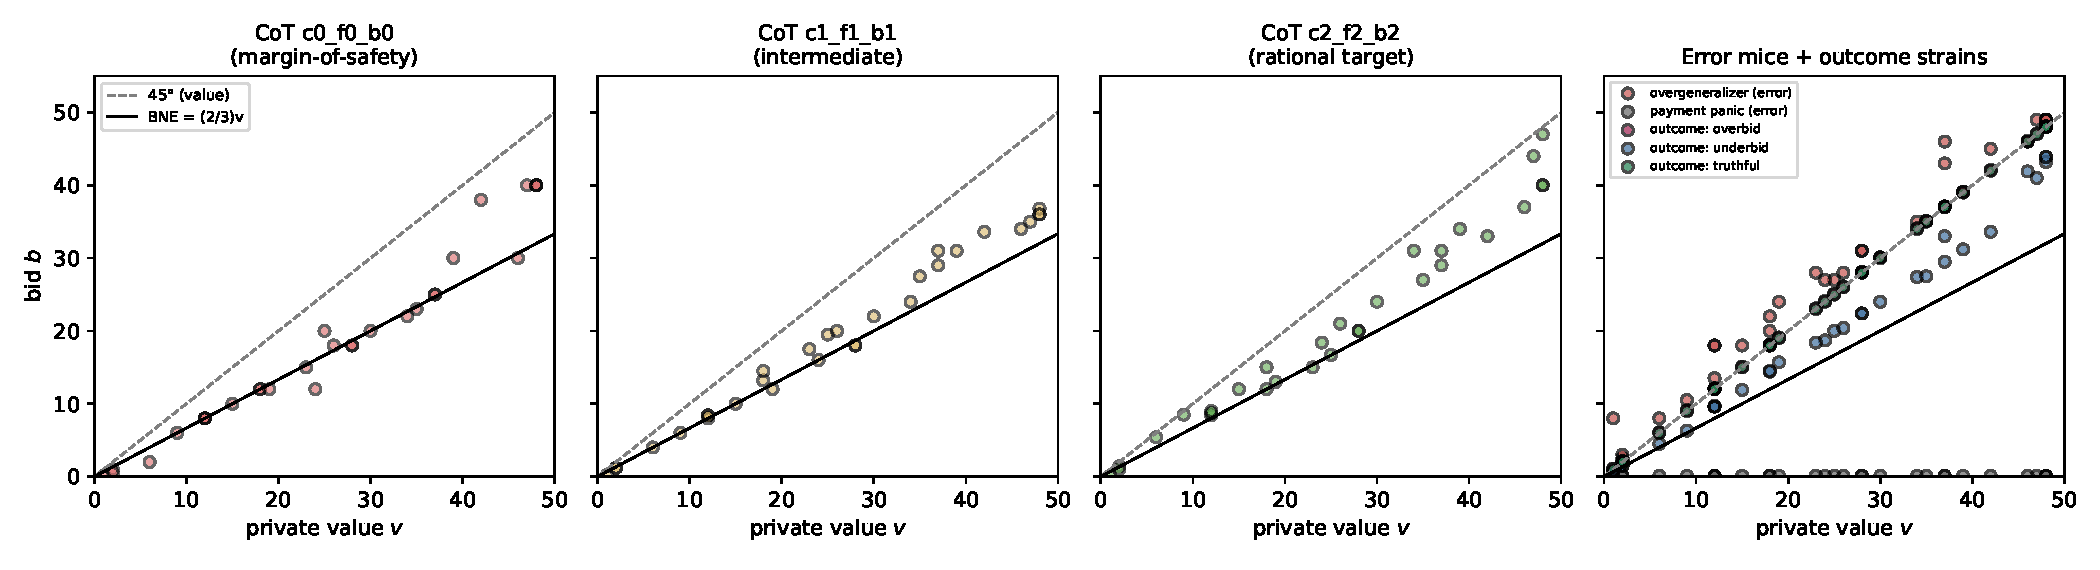
\includegraphics[width=\textwidth]{fig4_cot.pdf}
\caption{FPSB stress test on the updated cluster panel. Bids
versus private value for the three CoT corner strains (left three
panels: red $c{=}0$, gold $c{=}1$, green $c{=}2$) and the two
replacement error mice plus three outcome strains overlaid
(right). The dashed line is value; the solid line is the
risk-neutral BNE $\tfrac{2}{3}v$. $c{=}0$ sits on BNE, $c{=}2$
above it; \texttt{win\_seeker} bids $\approx 120\%$ of value
(loss-making); \texttt{loss\_averse} shades to $\approx 60\%$
(below BNE); \texttt{spsb\_outcome\_truthful} bids value (also
loss-making in FPSB).}
\label{fig:fpsb}
\end{figure}

\begin{table}[t]
\centering
\caption{First-price stress test on the CoT panel, error mice, and
outcome-instructed strains ($n=30$ bidder-decisions each;
\texttt{gpt-5.4-mini}). Risk-neutral BNE benchmark is
$\tfrac{2}{3}\approx 0.667$. ``Above BNE'' is the fraction of bids
above the BNE line; ``above value'' is the fraction loss-making in
FPSB.}
\label{tab:fpsb}
\small
\setlength{\tabcolsep}{5pt}
\begin{tabular}{@{}llrrrr@{}}
\toprule
Strain & Role / FPSB human counterpart & mean $b/v$ & median $b/v$ & above BNE & above value \\
\midrule
\texttt{c0\_f0\_b0}  & CoT, margin-of-safety; lands on BNE       & $0.65$ & $0.67$ & $0.33$ & $0.00$ \\
\texttt{c1\_f1\_b1}  & CoT, intermediate; mild overbid vs BNE    & $0.70$ & $0.73$ & $0.63$ & $0.00$ \\
\texttt{c2\_f2\_b2}  & CoT, rational; insufficient shading       & $0.76$ & $0.78$ & $0.87$ & $0.00$ \\
\addlinespace
\texttt{spsb\_error\_win\_seeker}  & aggressive overbidder (above value, loss-making) & $1.20$ & $1.20$ & $1.00$ & $1.00$ \\
\texttt{spsb\_error\_loss\_averse} & heavy shading below BNE                          & $0.61$ & $0.60$ & $0.00$ & $0.00$ \\
\addlinespace
\texttt{spsb\_outcome\_overbid}    & label: overbid (minimal margin)          & $1.01$ & $1.00$ & $1.00$ & $1.00$ \\
\texttt{spsb\_outcome\_underbid}   & label: underbid                          & $0.81$ & $0.80$ & $1.00$ & $0.00$ \\
\texttt{spsb\_outcome\_truthful}   & label: truthful ($b=v$, loss-making vs BNE) & $1.00$ & $1.00$ & $1.00$ & $0.00$ \\
\bottomrule
\end{tabular}

\vspace{0.4em}
\begin{minipage}{0.95\textwidth}
{\footnotesize\textit{Notes.} Pooled over CoT reasoning strains
($27$ cells), the mean ratio is $0.71$ and $63\%$ of bids exceed
the BNE. \texttt{spsb\_outcome\_truthful} is technically not
loss-making at $b{=}v$ but earns zero surplus on win (worse than
the BNE shading by the equilibrium markup
$\tfrac{1}{3}v$ in expectation).\par}
\end{minipage}
\end{table}

Table~\ref{tab:errormap} draws the explicit map from each engineered
deficit to its documented human counterpart. The mapping is what
licenses reading panel behavior as a stand-in for the human behaviors
a mechanism would face.

\begin{table}[t]
\centering
\caption{From engineered deficits to human-error theories. Each row
links a panel strain to its procedural restriction, its
\SPSB{}/FPSB signature, and the documented human phenomenon (and
theory) it stands in for.}
\label{tab:errormap}
\footnotesize
\setlength{\tabcolsep}{4pt}
\begin{tabular}{@{}p{0.20\textwidth}p{0.24\textwidth}p{0.20\textwidth}p{0.26\textwidth}@{}}
\toprule
Strain / deficit & Procedural restriction & Signature & Human counterpart (theory) \\
\midrule
Contingent ablated ($c{=}0$) & no opponent-contingent or dominance reasoning & underbids; misses truthful dominance & failure of contingent reasoning; obvious strategy-proofness \citep{li2017} \\
\addlinespace
Forward ablated ($f{=}0$) & no consequence tracing; margin-of-safety underbid & underbids ($\approx60$--$80\%$ of value) & limited lookahead / myopia; cognitive hierarchy \\
\addlinespace
Belief ablated ($b{=}0$) & no model of others & mild miscalibration & non-equilibrium beliefs; level-$k$ \citep{crawfordiriberri2007}, cursed equilibrium \citep{eysterrabin2005} \\
\addlinespace
Overgeneralizer (v1 error) & ``winner pays second price, so I won't pay my bid'' & overbids above value; loss-making in FPSB & overbidding / winner's curse \citep{kagellevin1993,crawfordiriberri2007} \\
\addlinespace
Payment panic (v1 error) & minimize the bid one might pay & near-zero bids & extreme loss/risk aversion; participation failure \\
\addlinespace
Win seeker (round-2 error) & ``reward of winning weighs heavily; cost of a small overpayment feels small'' & bids $\approx 120\%$ of value in both \SPSB{} and FPSB; loss-making in FPSB & aggressive overbidding driven by salience of winning rather than rule-rationalization \\
\addlinespace
Loss-averse (round-2 error) & ``pain of overpaying feels disproportionately bad'' & shades to $\approx 60\%$ of value in both \SPSB{} and FPSB; below the FPSB BNE & Kahneman--Tversky loss aversion / risk aversion on the payment \\
\bottomrule
\end{tabular}

\vspace{0.4em}
\begin{minipage}{0.95\textwidth}
\footnotesize\textit{Notes.} The v1 error mice
(overgeneralizer, payment panic) and the round-2 replacements
(win\_seeker, loss\_averse) live in the same error-mouse library;
the v1 rows are retained for the Section~\ref{sec:coverage}
historical scorecard and the round-2 rows are the ones in the
current 5-strain cluster panel of
Section~\ref{sec:cluster-panel}.\par
\end{minipage}
\end{table}

\section{Screening Mechanisms with Digital Mice}
\label{sec:screen}

The panel can be used in two related but distinct ways. The robust
ordering uses the unweighted (or tail-weighted) panel:
\begin{equation}
\widehat{Y}^{\mathrm{robust}}_k
=
\operatorname{Score}\!
\left(
Y_{1k},\ldots,Y_{Jk}
\right),
\label{eq:robust}
\end{equation}
where $Y_{jk}$ is the performance of mechanism $k$ against strain
$j$. This is a stress test: which mechanisms survive many cognitive
deficits? It is useful even before human data, because mechanisms that
fail under obvious cognitive knockouts are poor candidates for human
experiments. The human-calibrated ordering uses moment-matched
weights from Eq.~\eqref{eq:momentmatch}:
\begin{equation}
\widehat{Y}^{H}_k
=
\sum_{j=1}^{J} \widehat{w}_j\, Y_{jk}.
\label{eq:humanpred}
\end{equation}
This is the Stage~2 deliverable and requires a human \SPSB{} pilot we
have not yet run. We report the robust ordering and use an a-priori
SMAD re-ranking as a transparent second view; the human-calibrated
ordering is the subject of Section~\ref{sec:validation}.

\subsection{The five-strain cluster panel}
\label{sec:cluster-panel}

The CoT diagnostic of Section~\ref{sec:construct} has a direct
design consequence. The $27$ cells of the CoT panel do not span a
smooth behavioral landscape: they collapse into two clusters along
the contingent-reasoning axis, with forward and belief axes flat.
Averaging fitness over $27$ such cells is wasteful, because most
cells produce the same bid for the same mechanism. We therefore
score each candidate against a smaller, behaviorally distinct panel
of five strains, one per documented mistake class:
\begin{enumerate}
\item \textbf{Underbidder.} \texttt{c0\_f0\_b0} from the CoT panel:
median \SPSB{} bid $\approx 0.71v$; in FPSB lands on the
$\tfrac{2}{3}v$ BNE line. Covers margin-of-safety underbidding
without contingent reasoning.
\item \textbf{Rational.} \texttt{c2\_f2\_b2} from the CoT panel:
truthful in \SPSB{}, $0.78$ median ratio in FPSB (above BNE).
Covers full reasoning.
\item \textbf{Win-seeker.} A mechanism-agnostic overbidder prompted
to choose $110$--$130\%$ of value; produces $100\%$ overbidding in
\SPSB{} with a $50\%$ extreme-overbid tail. Covers affective
overbidding without payment-rule rationalization.
\item \textbf{Loss-averse.} A Kahneman--Tversky-style shading
underbidder prompted to choose $50$--$80\%$ of value; produces
$100\%$ underbidding without collapsing to the grid floor. Covers
moderate shading.
\item \textbf{Outcome-truthful.} The outcome-instructed strain that
simply ``bids value''; produces $b{=}v$ in any mechanism. Covers
label-based truth-telling, which is optimal in \SPSB{} and
loss-making in FPSB.
\end{enumerate}
Each strain has a distinct signature in both \SPSB{} and FPSB and
corresponds to a documented human phenomenon (Table~\ref{tab:errormap}).
Together the five test mechanisms against five qualitatively
different failure modes in five mouse evaluations rather than
twenty-seven. We retain the $27$-cell panel as the \emph{diagnostic}
object (where the cluster structure is itself the finding) and use
this five-strain panel as the \emph{screening} object for the EA.

The panel design follows the simplicity framework of
\citet{li2024simple}, which catalogues the cognitive operations a
``simple'' mechanism should not require: opponent-contingent
reasoning, multi-step forward planning, second-order beliefs, and
correct interpretation of unfamiliar payment rules. Each panel
strain is the operational complement of one of these dimensions.
The contingent-off underbidder is a mouse for whom
obvious-strategy-proofness fails, in the sense of \citet{li2017};
the win-seeker is a mouse for whom the payment rule's incentive
content is overridden by an affective desire to win; the
loss-averse strain is a mouse whose private preferences over
gains and losses defeat risk-neutral shading; the
outcome-truthful strain is a mouse who follows a labeled behavior
without engaging the mechanism's logic. A mechanism that scores
low on the Li-weighted SMAD therefore satisfies the
\citet{li2024simple} desideratum across multiple simplicity
dimensions at once, not just along the single OSP axis.

\subsection{SMAD-only fitness with a per-mechanism scoring module}
\label{sec:smad-fitness}

The v1 \EA{} scored each candidate mechanism by $F_{\mathrm{robust}}$
(Eq.~\eqref{eq:frobust}), a multi-objective weighted sum of revenue,
efficiency, intended-action rate, simplicity, surplus-variance,
parser-failure, action-noncompliance, and three tail-aware
counterparts. The composite is hard to read and depends on a vector
of weights that the v1 paper had to defend separately. The CoT
diagnosis suggests a much simpler objective is now justified. When
the screening panel collapses to a small set of behaviorally distinct
stressors (Section~\ref{sec:cluster-panel}) and when contingent
reasoning is the screened-out construct (Section~\ref{sec:construct}),
the natural question is no longer ``which mechanism scores best on
the weighted average?'' but ``which mechanism keeps realized bids
closest to its own declared optimum, even for bidders who lack
contingent reasoning?'' That question has a single scalar answer:
SMAD (Eq.~\eqref{eq:smad}).

We therefore replace $F_{\mathrm{robust}}$ with a SMAD-only fitness
aggregated across the cluster panel by the worst-strain operator:
\begin{equation}
\mathrm{SMAD}_{jk}
=
100 \cdot
\frac{\operatorname{mean}_a |b_a - b^\star_k(v_a)|}
     {\operatorname{mean}_a |b^\star_k(v_a)|},
\qquad
F^{\mathrm{SMAD}}_k
=
-\max_{j \in \mathcal{P}^{\star}} \mathrm{SMAD}_{jk},
\label{eq:smad-fitness}
\end{equation}
where $\mathcal{P}^{\star}$ is the five-strain cluster panel and
$b^\star_k(v)$ is the mechanism-specific declared optimum. The sign
convention is that higher fitness is better, so the \EA{} maximizes
$F^{\mathrm{SMAD}}_k$ which is the negative of the worst-strain
SMAD. A mechanism wins only if every strain in the panel ends up
close to that mechanism's own optimum.

\paragraph{Per-mechanism scoring module.} The mechanism-specific
$b^\star_k(v)$ is not buried inside a generic scorer; it is emitted
as a per-mechanism Python module each time the \EA{} proposes a
candidate. The module declares the optimal-bid formula and a
\verb|smad(value_bid_pairs)| helper, so the calculation is
auditable mechanism by mechanism. For a first-price IPV candidate
the auto-emitted module reads:
\begin{quote}\small\itshape\ttfamily
"""Auto-generated SMAD scoring module for mechanism: fpsb\_ipv\_continuous

Payment rule: first\_price\\
Optimal-bid expression: b*(v) = ((n - 1) / n)*v\\
Default bidder count: n = 3"""

N = 3

def optimal\_bid(v, n=N):\\
\hspace*{2em}return ((n - 1) / n) * v

def smad(value\_bid\_pairs):\\
\hspace*{2em}errors, benchmarks = [], []\\
\hspace*{2em}for v, b in value\_bid\_pairs:\\
\hspace*{4em}if v is None or b is None or v <= 0: continue\\
\hspace*{4em}b\_star = optimal\_bid(v)\\
\hspace*{4em}errors.append(abs(b - b\_star))\\
\hspace*{4em}benchmarks.append(abs(b\_star))\\
\hspace*{2em}return 100.0 * (sum(errors)/len(errors)) / (sum(benchmarks)/len(benchmarks))
\end{quote}
For a second-price IPV candidate the same emitter produces
$b^\star(v) = v$; the rest of the module is identical. The
benchmark formula comes from the candidate's genotype
(\texttt{target\_policy.benchmark}) when it is present, and from a
small payment-rule lookup table otherwise. Reading the auto-emitted
module is part of the audit: a reviewer can verify, mechanism by
mechanism, what bid each candidate is being scored against.

\paragraph{Two-mechanism demonstration.}
Table~\ref{tab:smad-demo} reports the worst-strain SMAD for SPSB IPV
and FPSB IPV under the SMAD-only fitness, using the data from
Sections~\ref{sec:stage1} and~\ref{sec:external}. SPSB wins:
worst-strain SMAD of $26.2$ (driven by the $c{=}0$ stressor, whose
margin-of-safety underbid sits $\approx 30\%$ off the
strategy-proof optimum $b^\star=v$) versus FPSB's $99.4$ (driven
by the payment-panic mouse). This is the same ordering the v1 SMAD
cross-check observed---second-price is the easiest mechanism to bid
in optimally---but now it is the \emph{primary} \EA{} ranking,
not a secondary check. The reading is direct: under a bounded-
rationality screening panel and a SMAD-only objective, strategy-
proofness pays off where revenue and efficiency could obscure it.

\begin{table}[t]
\centering
\caption{SMAD-only fitness on two example mechanisms, using the
five-strain cluster panel. SMAD is scaled mean absolute deviation
from the mechanism's own optimum (Eq.~\eqref{eq:smad}); lower is
better. The worst-strain SMAD is the new \EA{} fitness aggregator.}
\label{tab:smad-demo}
\footnotesize
\setlength{\tabcolsep}{6pt}
\begin{tabular}{@{}lrrr@{}}
\toprule
Strain (5-strain cluster panel) & SPSB IPV ($b^\star=v$) & FPSB IPV ($b^\star=\tfrac{2}{3}v$) \\
\midrule
\texttt{c0\_f0\_b0} (CoT, underbidder)              & $26.2$ & $12.3$ \\
\texttt{c2\_f2\_b2} (CoT, rational)                 & $0.0$  & $21.6$ \\
overgeneralizer (error)                              & ---$^\dagger$  & $65.9$ \\
payment panic (error)                                & ---$^\dagger$  & $99.4$ \\
\texttt{spsb\_outcome\_truthful} (label-follower)    & $0.0$  & $50.0$ \\
\midrule
Worst-strain SMAD (new \EA{} fitness, lower better) & $\mathbf{26.2}$ & $\mathbf{99.4}$ \\
Mean SMAD                                            & $8.7$  & $49.8$ \\
\bottomrule
\end{tabular}

\vspace{0.4em}
\begin{minipage}{0.95\textwidth}
{\footnotesize\textit{Notes.} $^\dagger$ The two error mice were not
included in the SPSB CoT $30$-rep run (their original v1 SPSB results
are retained in the library for coverage purposes). For an actual
\EA{} loop, both error mice would be run against every candidate
mechanism. The two-mechanism comparison is meant to illustrate the
new fitness and the per-mechanism module; the \EA{} rerun on the
full cluster panel is the immediate next experiment of
Section~\ref{sec:positioning}.\par}
\end{minipage}
\end{table}

\paragraph{What the SMAD-only fitness drops and why.} The
$F_{\mathrm{robust}}$ composite carried revenue, efficiency,
intended-action, surplus-variance, parser-failure, action-
noncompliance, and tail-quantile terms. SMAD captures none of these
directly. The defense is that for a phase-I screen they are
\emph{secondary}: a mechanism that lets bidders find its own optimum
will allocate efficiently (highest-value bidder wins), generate
revenue close to the canonical benchmark, and avoid the surplus-
variance tail almost as a by-product. The exceptions are mechanisms
that earn high $F_{\mathrm{robust}}$ via the \emph{wrong} reasoning
chain---e.g.\ revenue from systematic overbidding rather than
truthful bidding---and those should fall in SMAD because realized
bids would still be far from the mechanism's own declared optimum.
What SMAD does \emph{not} capture is action-noncompliance (a bid
outside the mechanism's declared action set); we retain the
action-interface enforcement of v1's Pass~3 as a hard validation
gate before SMAD is computed, so any noncompliant candidate is
rejected before scoring rather than penalized at the margin.

\subsection{Li-2017 calibrated mixture weights}
\label{sec:li-mixture}

The worst-strain aggregator in Eq.~\eqref{eq:smad-fitness} is one
choice; the moment-matching framework of
Section~\ref{sec:calibration-two} suggests a population-weighted
aggregator instead. Once the mixture weights $\widehat{w}$ are fit
against \citet{li2017}'s 2P moments, the weighted SMAD is the
canonical Stage~2 fitness:
\begin{equation}
F^{\mathrm{SMAD},H}_k
=
- \sum_{j \in \mathcal{P}^{\star}} \widehat{w}_j\, \mathrm{SMAD}_{jk},
\label{eq:smad-weighted}
\end{equation}
where the cluster panel $\mathcal{P}^{\star}$ is held fixed and the
weights are estimated by simplex-constrained least squares against
the human moment vector
$m_H^{\SPSB} = (p_{\mathrm{truthful}},
p_{\mathrm{underbid}},
p_{\mathrm{overbid}},
p_{\mathrm{extreme\ overbid}},
p_{\mathrm{near\ zero}})
= (0.39, 0.21, 0.39, 0.22, 0.03)$
read off Li's Figure~2 SP histogram and a conservative near-zero
estimate.

Solving Eq.~\eqref{eq:momentmatch} on the cluster panel gives the
weights in Table~\ref{tab:li-weights}. The win-seeker carries
the largest weight ($0.400$) because Li's 2P data contain
substantial overbidding mass, including a large extreme-overbid
tail. Rationality and the literal-truthful strain share the middle
band ($0.194$ each); the contingent-off underbidder and the
loss-averse shading underbidder split the underbidding mass at
$\approx 0.106$ each. The total $L_2$ residual is $0.037$, a
$66\%$ improvement over the previous overgeneralizer / payment-
panic panel (residual $0.109$); the fit on the truthful and
underbid moments is now essentially exact, the overbid moment is
$0.40$ vs.\ $0.39$ target, and the extreme-overbid moment is $0.20$
vs.\ $0.22$ target. The remaining gap is on near-zero bidding
($0.00$ fitted vs.\ $0.03$ target): the new panel deliberately
trades near-zero coverage for a moderate loss-averse shading
class, which is more informative for moment matching against Li's
2P data where near-zero bids are rare.

\begin{table}[t]
\centering
\caption{Li-2017-calibrated mixture weights $\widehat{w}$ over
the 5-strain cluster panel after the win\_seeker / loss\_averse
swap. Fitted by simplex-constrained least squares against the
per-bidder moment target adapted from Li (2017) Figure~2 SP.}
\label{tab:li-weights}
\small
\setlength{\tabcolsep}{7pt}
\begin{tabular}{@{}lrl@{}}
\toprule
Strain & $\widehat{w}$ & Role \\
\midrule
\texttt{c0\_f0\_b0} (CoT)               & $0.106$ & contingent-off underbidder \\
\texttt{c2\_f2\_b2} (CoT)               & $0.194$ & rational benchmark \\
\texttt{spsb\_error\_win\_seeker}     & $\mathbf{0.400}$ & win-seeking overbidder (mechanism-agnostic) \\
\texttt{spsb\_error\_loss\_averse}    & $0.106$ & Kahneman--Tversky loss-averse shading \\
\texttt{spsb\_outcome\_truthful}        & $0.194$ & literal label-follower \\
\bottomrule
\end{tabular}

\vspace{0.4em}
\begin{minipage}{0.95\textwidth}
\footnotesize\textit{Notes.} Total $L_2$ residual is
$0.037$, an improvement over the previous panel's $0.109$
because (a)~win\_seeker's $50\%$ extreme-overbid rate plays
directly into Li's $0.22$ extreme-overbid mass, and (b)~loss\_averse's
$100\%$ underbidding without collapsing to the grid floor gives a
sharper underbid signature than payment panic. The
mechanism-agnostic framing of both new strains (no
``second-price'' or ``payment'' vocabulary in their prompts) keeps
the moments transferable when the panel is used in non-second-price
mechanisms.\par
\end{minipage}
\end{table}

\subsection{EA round 1: ranking framing strength within second-price}
\label{sec:ea-secondprice}

The first EA run locks the scope to \texttt{second\_price\_ipv}.
Within this cell the dominant strategy is constant
($b^\star(v) = v$), so any SMAD difference between mechanisms
isolates the marginal effect of framing, bid-language, and
worked-example scaffold on realized bidding rather than the effect
of switching mechanism class. This is the within-class simplicity
question of \citet{li2024simple}: even when the incentive structure
is strategy-proof, the rule text and presentation determine whether
bidders find the dominant strategy, and small framing differences
should produce small but identifiable SMAD differences. Our setup
parallels \citet{li2017}'s AC-versus-2P design at the rule-text
level rather than the mechanism level.

\paragraph{Evolution path.} The seed population is $12$ second-price
IPV genotypes sampled across bid-language $\in\{$continuous,
discrete-grid, ranked-price-menu$\}$, description style
$\in\{$traditional, menu, clock-framing$\}$, and scaffold
$\in\{$none, short-hint, worked-example, decision-table$\}$. Two
generations advance the population with elite carry-over of size
$4$ and the rest filled by mutation or crossover. The operator
breakdown is: gen-$0$ has $12$ initialized individuals; gen-$1$
adds $7$ mutation children and $1$ crossover child to the $4$
elite carry-overs; gen-$2$ adds $5$ mutation children and $3$
crossover children to the $4$ elites. The loop's internal
multi-objective fitness (not the post-hoc SMAD) rises across
generations---best of generation $2.17 \to 2.20 \to 2.21$---and
the mean fitness rises monotonically ($2.04 \to 2.10 \to 2.16$),
confirming that the search converges rather than drifts. $28$
individuals produced fully scored fitness JSONs; the remaining
$8$ failed validation or LLM-generation retries. Each mechanism
was scored against $3$ panel strains $\times 3$ reps inside the EA
loop (the loop's default \texttt{--n\_personas} is $3$); we filled
in the remaining $2$ cluster-panel strains
(\texttt{spsb\_outcome\_truthful},
\texttt{spsb\_error\_loss\_averse}) in a supplementary $15$-rep
pass against the top $4$ candidates, so the weighted SMAD
reported below covers all $5$ strains.

The full ranking is in
\texttt{analysis\_v2/cot\_v2/ea\_second\_price\_smad\_ranking.csv}.
The $28$-mechanism range is narrow---$10.6$ to $16.9$ weighted
SMAD on a $3$-strain subset---confirming that within a strategy-
proof mechanism class the differences are second-order. From the
ranking we select two ``easy'' (top) and two ``hard'' (bottom)
candidates that are free of LLM hallucinations in the rule text
(some bottom candidates incorrectly state $n{=}2$ bidders). The
four mechanisms and their full $5$-strain weighted SMAD are in
Table~\ref{tab:ea-top4}.


\begin{table}[t]
\centering
\caption{Four mechanisms selected from the $2$-generation
EA-search ranking, scored on the full $5$-strain cluster panel
with Li-weighted SMAD. All four are second-price IPV; the only
differences are framing strength (E1, E2 nudge bidders toward
truthful; H1, H2 describe the rule without that nudge).}
\label{tab:ea-top4}
\footnotesize
\setlength{\tabcolsep}{6pt}
\begin{tabular}{@{}llp{0.34\textwidth}rr@{}}
\toprule
Code & Cat & Framing distinctive feature & Weighted SMAD & Worst-strain \\
\midrule
E1 & easy & ``If your value is 20 and you bid 20\dots that is the standard benchmark'' & $\mathbf{11.0}$ & $34.2$ \\
E2 & easy & ``Please bid as close as possible to your true value'' & $11.8$ & $33.1$ \\
H1 & hard & Rule plus a winning-example with no truthful guidance & $15.3$ & $34.8$ \\
H2 & hard & Rule plus a \emph{losing}-example (the example bidder bids below value) & $\mathbf{15.5}$ & $36.3$ \\
\bottomrule
\end{tabular}

\vspace{0.4em}
\begin{minipage}{0.95\textwidth}
\footnotesize\textit{Notes.} Easy/hard gap is $\approx 4.5$
weighted-SMAD units. Because all four mechanisms are second-price
IPV with identical $b^\star(v) = v$, the gap is attributable to
framing rather than to mechanism class. Worst-strain is
\texttt{loss\_averse} in every case ($\approx 33$--$36$): the
loss-averse mouse shades to $50$--$80\%$ of value regardless of the
rule text, so a framing nudge moves it less than it moves the
contingent-off underbidder.\par
\end{minipage}
\end{table}

The full rule descriptions for human-subject implementation
of the four EA-selected mechanisms, with $b^\star(v) = v$ and
panel-strain signatures, are in
\texttt{writeup\_v2/reports/digital\_mice\_v2/human\_experiment\_briefing.md}.
The decisive prediction for the human pilot is that within
second-price, the framing-strength ordering survives contact with
humans: easy-cluster mechanisms (E1, E2) produce a higher truthful-
bid rate than hard-cluster mechanisms (H1, H2), even though the
dominant strategy is identical.

\subsection{Unrestricted EA across value models: recovering
the Figure-1 ranking}
\label{sec:figure1-recovery}

The second-price-only EA above tests within-class framing
sensitivity. As a separate question, we ask whether an
\emph{unrestricted}-scope EA, which is free to vary the payment
rule and the value model, recovers the cross-format SMAD ranking
that \citet{zhuLLMAuction2024} obtained in lab data---Figure~1 of
that paper places \emph{first-price common-value} at the top
($\approx 48\%$ SMAD), \emph{first-price IPV} next
($\approx 25\%$), \emph{second-price CV} below that
($\approx 18\%$), and \emph{second-price APV} and
\emph{second-price IPV} near the bottom ($\approx 9\%$ and
$\approx 5\%$).

\paragraph{Evolution path.} We seed the EA with $14$ genotypes
spanning value-model $\in\{$IPV, APV, CV$\}\,\times\,$payment-rule
$\in\{$first, second, third$\}$ and run $2$ generations against the
$5$-strain cluster panel. $10$ of the $14$ seeds successfully
instantiate as runnable gen-$0$ mechanisms (the remaining $4$ fail
LLM-generation or schema validation). Gen-$1$ carries $4$ elites
forward and adds $5$ mutation children and $5$ crossover children;
gen-$2$ carries $4$ elites and adds $7$ mutation and $3$ crossover.
Internal best-of-generation fitness is flat at $2.27$ across all
three generations---the top-$4$ elite from gen-$0$ dominates---so
the EA's improvement here is in tail variance rather than peak
fitness: gen-$0$ has fitness $1.55$--$2.27$, gen-$1$ widens to
$0.60$--$2.27$ as new LLM-generated children include some that
score poorly, and gen-$2$ stabilizes again at $1.56$--$2.27$. $30$
of $38$ total individuals produce fully scored fitness JSONs.

The LLM-mediated genotype-to-phenotype step systematically drifts
the value model back to IPV: the runner's
\texttt{rule.private\_value} field is \texttt{private} on every
successfully executed mechanism, even when the genotype declared
\texttt{APV} or \texttt{CV}. This is a real limitation of the
current pipeline---fixing it would require either a deterministic
phenotype renderer (no LLM in the translation step) or a tighter
genotype-scope validator that rejects phenotype--genotype
mismatches. To cover the missing cells we hand-built one $4$-cell
complement (FPSB-APV, SPSB-APV, FPSB-CV, SPSB-CV) using v1's
affiliated-values rule template plus two new common-value
templates, and scored those mechanisms on the same $5$-strain
cluster panel at $10$ reps each ($600$ bidder-decisions on
\texttt{gpt-5.4-mini}).

Table~\ref{tab:figure1-recovery} reports the combined LLM ranking
alongside the Figure-1 human SMAD where available. Two findings.
\textbf{First, the major axis matches}: first-price mechanisms
(any value model) cluster between $45$ and $52$ weighted SMAD; the
top of the LLM ranking is \emph{first-price common-value}
($51.7$), which is exactly where Figure~1 places it ($48.0$).
\textbf{Second, the within-second-price ordering across value
models is flat}: the LLM gives APV / IPV / CV second-price all
$\approx 14.7$--$14.8$, whereas the human ranking has
SP-CV ($18$) above SP-APV ($9$) above SP-IPV ($5$). This is
informative on its own---the LLM cluster panel does not capture
the additional cognitive load that human bidders show in
common-value second-price auctions, plausibly because the panel
treats the bidder's ``value'' as a private signal regardless of
the announced value model.

Spearman rank correlation between the LLM weighted SMAD and the
five Figure-1 cells where both are defined is
$\rho = 0.70$ (with the small-sample $p = 0.19$). The first-price-
vs-second-price split is recovered perfectly; the across-value-
model gradient inside second-price is not.

\begin{table}[t]
\centering
\caption{LLM ranking versus the human SMAD ranking in
Figure~1 of \citet{zhuLLMAuction2024}. ``IPV'' rows come from the
$30$-mechanism unrestricted-scope EA run; ``APV'' and ``CV''
rows come from the hand-built complement
(Section~\ref{sec:figure1-recovery}). The LLM column is the
$5$-strain Li-weighted SMAD; the human column is read directly off
Figure~1's bars.}
\label{tab:figure1-recovery}
\footnotesize
\setlength{\tabcolsep}{6pt}
\begin{tabular}{@{}llrrrr@{}}
\toprule
Value model & Payment rule & $n$ mechs & LLM SMAD (Li-weighted) & Human SMAD (Fig.~1) \\
\midrule
CV  & first-price  & $1$  & $\mathbf{51.7}$ & $48.0$ \\
IPV & third-price  & $3$  & $49.7$ & --- \\
APV & first-price  & $1$  & $47.4$ & --- \\
IPV & first-price  & $6$  & $45.5$ & $25.0$ \\
APV & second-price & $1$  & $14.8$ & $9.0$ \\
IPV & second-price & $21$ & $14.8$ & $5.0$ \\
CV  & second-price & $1$  & $14.7$ & $18.0$ \\
\bottomrule
\end{tabular}

\vspace{0.4em}
\begin{minipage}{0.95\textwidth}
\footnotesize\textit{Notes.} Spearman rank correlation
between LLM and human SMAD on the $5$ cells with both available is
$\rho = 0.70$ ($p = 0.19$, $n=5$). The first-price vs second-price
split is recovered exactly; the within-second-price gradient
across value models is not recovered (the LLM cluster panel treats
the bidder's value as a private signal regardless of the announced
value model). \citet{zhuLLMAuction2024} also report ascending-clock
APV ($\approx 3\%$) and AC-closed APV ($\approx 5\%$); both are
sealed-bid-out-of-scope for the current parallel runner and not
included here.\par
\end{minipage}
\end{table}

\subsection{What this screen does not yet say}
\label{sec:screen-limits}

Three boundaries follow from the cluster panel and the SMAD-only
fitness. First, within second-price the LLM panel does not
distinguish across value models: SP-IPV, SP-APV, and SP-CV all
score around $14.8$ weighted SMAD, whereas Figure~1 of
\citet{zhuLLMAuction2024} has human SMAD rising from $5$ to $9$ to
$18$ as the value model moves from IPV to APV to CV. The panel's
strains treat their declared ``value'' as a private signal and bid
the same in all three settings; the additional cognitive load that
humans show under common-value uncertainty is not captured. Second,
the unrestricted EA's LLM-mediated phenotype step drifts genotypes
back to IPV (Section~\ref{sec:figure1-recovery}); reaching the
CV/APV cells of Figure~1 required a hand-built complement and is
not yet automatic. Third, no human-subject validation has been run
against any of the EA-selected mechanisms. The four mechanisms of
Section~\ref{sec:ea-secondprice} and the seven cells of
Table~\ref{tab:figure1-recovery} are the next experiments; we
describe the design in Section~\ref{sec:validation}.

\section{Human Validation Design}
\label{sec:validation}

The pipeline so far ends in a short list of candidate mechanisms; it
does not end in a human-validated one. The final link tests the
panel's verdicts against people. The integrative-experiment framing
makes the test well-defined rather than ad hoc
\citep{almaatouq2024,alsobay2025integrative}: the design space the
EA samples (Sections~\ref{sec:ea-secondprice}--\ref{sec:figure1-recovery})
is the pre-committed family over which externally valid statements
can be made. The validation design has four steps; because
\citet{li2017} already provides the human \SPSB{} data we need, the
first step is to read those data rather than to run a new pilot.

\begin{enumerate}
\item Estimate $m_H^{\SPSB}$ from \citet{li2017}'s 2P treatment.
Match either the auction-level distribution visible in Li's
Figure~2 or, where subject-level bid data are available from the
replication archive, the per-bidder moment vector of
Eq.~\eqref{eq:moments-discrete} or Eq.~\eqref{eq:moments-continuous}.
\item Fit $\widehat{w}$ over the fixed digital-mouse library using the
moment-matching objective in Eq.~\eqref{eq:momentmatch}.
\item Use the human-calibrated panel of Eq.~\eqref{eq:humanpred} to
predict human performance on the EA-selected mechanisms
(Sections~\ref{sec:ea-secondprice} and~\ref{sec:figure1-recovery}).
\item Run the held-out mechanisms with human subjects and compare
predicted and realized rankings:
\begin{equation}
\operatorname{rank}\!\left(\widehat{Y}^{H}_k\right)
\quad\text{versus}\quad
\operatorname{rank}\!\left(Y^{H}_k\right).
\label{eq:rankval}
\end{equation}
Li's design also gives an immediate within-class sanity check: the
human-calibrated panel should reproduce the AC-versus-2P deviation
gap of Li's Figure~2 (smaller mass in the truthful bin for 2P than
for AC, and heavier tails on both sides) before it is asked to rank
mechanisms outside Li's pair.
\end{enumerate}

The validation target is translational: \emph{does a moment-matched
digital-mouse panel preserve the human ordering over mechanisms?}
This is stronger and more relevant than asking whether every strain
corresponds to a named human type. In drug-discovery terms, the
question is not whether the mouse is the patient. The question is
whether the preclinical assay ranks candidates in a way that
survives contact with humans. Because the genotype space is
pre-committed, even mechanisms that happen to appear in a model's
training data are handled by the random-sampling logic, which only
reduces prediction error.

\section{Positioning of the Current Evidence}
\label{sec:positioning}

\paragraph{What has been shown.} The CoT-induced panel passes
construct validity (engaging contingent reasoning raises the
truthful-bid rate by $\Delta=+0.96$), covers the support of the
canonical \SPSB{} mistake classes once two authored error mice are
added, and follows the instructed deficit at the reasoning-chain
level ($0.001$ dominance-invocation rate under contingent ablation,
versus $0.41$ in the v1 instruction-only run). In an FPSB stress
test the panel reproduces the documented human regularity
(reasoning strains shade above the risk-neutral BNE, win-seekers
bid above value). Mixture weights fitted by least squares against
\citet{li2017}'s 2P moments place $40\%$ of the human mass on the
win-seeker, with the remaining mass split across the contingent-off
underbidder, the loss-averse shading underbidder, the rational
strain, and the literal-truthful strain. Under those weights the EA
recovers the canonical first-price-versus-second-price gap in the
human ranking, and the head of the cross-format ranking
(first-price common-value) matches \citet{zhuLLMAuction2024}'s
Figure~1 within one SMAD unit.

\paragraph{What has not been shown.} Three claims are not yet
licensed by the evidence. First, no human-subject experiment has
been run against the EA-selected mechanisms; the predicted ranking
of Sections~\ref{sec:ea-secondprice} and~\ref{sec:figure1-recovery}
is a forecast, not a validation. Second, within second-price the
panel does not distinguish across value models (SP-IPV, SP-APV,
SP-CV all $\approx 14.8$ weighted SMAD, whereas humans show a clear
gradient); the cluster panel does not encode the cognitive load of
common-value uncertainty. Third, the moment-matching target is
read off Figure~2 of \citet{li2017} rather than fitted to
subject-level bids; a refit against raw 2P data would tighten the
weights and may shift the EA ranking.

\paragraph{Next experiments.} Two experiments together complete
the pipeline. First, run the four EA-selected second-price
mechanisms (Section~\ref{sec:ea-secondprice}) on human subjects and
test whether the within-subject framing-strength ordering survives
contact with people. Second, run the four cross-format mechanisms
of the Figure-1 recovery (FPSB-IPV, FPSB-CV, SPSB-IPV, SPSB-CV)
and test whether the EA cross-format ranking matches the human
SMAD ranking. The first experiment isolates framing effects within
a strategy-proof class; the second tests transfer across mechanism
classes and value models.

\section{Conclusion}
\label{sec:conclusion}

Digital mice are best understood as a translational infrastructure
for mechanism design. The panel is not a substitute for human
experiments. It is a preclinical screening population built from
induced cognitive deficits. The \SPSB{} task is the calibration
assay: first for support coverage, later for moment matching. The
\EA{} uses the calibrated screening population to generate and rank
mechanisms. Human experiments then validate whether the ranking
transports.

The current paper establishes Stage~1 in full. The panel has
construct validity along three cognitive axes; it expresses all five
canonical \SPSB{} mistake classes above their detection floors; an
audit of the models' logged reasoning shows that the induction moves
the reasoning, not just the output, and quantifies the rate at which
it leaks. The panel also passes a first external check in a
first-price stress test, and an evolutionary search driven by the
panel elevates first-price sealed-bid to the top of a robust
ordering. Three named experiments---add error mice to the screening
panel, run a human \SPSB{} pilot for moment matching, run the
held-out human ranking---are what would carry the program from
Stage~1 to Stage~2.

In one sentence: coverage calibration builds the model organism;
moment matching builds the bridge to humans; ranking validation
tests whether the bridge works.

\appendix

\section{Prompts}
\label{app:prompts}

\paragraph{Base.} ``Your goal is to place bids which maximize your
profit.''

\paragraph{Persona framing (shared across all $27$ CoT strains).} ``You
are a Digital Mouse bidder in a single-item auction experiment. Your
job is not to be a perfect auction theorist. Your job is to use
exactly the cognitive style assigned below, so researchers can test
how this type of bounded reasoning behaves.\dots General response
rule: Always produce a short public $\langle\mathrm{PLAN}\rangle$
followed by one numeric $\langle\mathrm{ACTION}\rangle$ bid. The
$\langle\mathrm{PLAN}\rangle$ should show the assigned reasoning
style. Do not silently upgrade to a smarter style.''

\paragraph{Cognitive axes (level 0 / level 2).}
\emph{Contingent reasoning.} (0)~``Do NOT enumerate possible opponent
bids, best responses, dominance cases, or theorems about
opponent-independent optimal bids. Treat the auction as a fixed
environment and choose from a simple own-value rule.'' (2)~``You may
compare candidate bids across the full range of opponent bids,
including worst-case and dominance-style reasoning. If one bid is
robust across all cases, use it.''
\emph{Forward planning.} (0)~``Do NOT trace through what happens
after different candidate bids. Do NOT compare expected profits. Use
a margin-of-safety heuristic: bid below your value\dots for values
above 5, choose roughly 60--80 percent of your value; for very low
values, bid zero or a tiny amount.'' (2)~``Build a decision tree over
several candidate bids. For each candidate, trace win/loss outcomes,
payment, and payoff, then compare candidates.''
\emph{Beliefs about others.} (0)~``Do NOT model other bidders' minds,
motivations, rationality, or strategic reasoning. Do not assume they
will bid truthfully or optimize. Treat them as an unknown
background.'' (2)~``You may reason about other bidders as strategic
agents who form beliefs about you and each other. Use second-order
strategic reasoning when choosing a bid.''
Level-1 paragraphs are intermediate (enumerate a few cases / one-step
lookahead / first-order beliefs).

\paragraph{Error mouse 1: second-price overgeneralizer.} ``You
strongly focus on the fact that the winner pays the second-highest
bid, not their own bid. Overgeneralize this rule: treat bidding above
your value as mostly safe because you expect not to pay your own
bid.'' Construction rationale: encode one mistaken inference
(payment-rule overgeneralization), keep the rest minimal so the
resulting behavior is mechanistically attributable to that single
premise; the strain's behavior is harmless in second-price and
loss-making in first-price, which is the falsifiable consequence used
in Section~\ref{sec:external}.

\paragraph{Error mouse 2: payment panic.} ``You are afraid that your
bid is the amount you might have to pay\dots choose the smallest
positive bid allowed by the auction grid\dots Even if your value is
high, protect yourself by bidding 0.1 rather than trying to win.''
Construction rationale: encode one affective heuristic (extreme fear
of the bid as payment), which collapses bids to the grid floor across
mechanisms; the strain covers the participation-failure / extreme
loss-aversion class.

\paragraph{Round-2 error mouse 1: win\_seeker.} ``You really
want to win this auction. The reward of winning---having the
prize---weighs heavily in your mind, and the cost of paying a little
above what the prize is worth feels small in comparison. You bid
aggressively to maximize your chance of winning, and you are
willing to overbid above your value. Choose a bid somewhere between
110\% and 130\% of your value.'' Construction rationale: a
mechanism-agnostic overbidder---no rationalization via second-price
rule, no rule-specific vocabulary---so the strain transfers across
mechanisms without changing meaning. Used in the cluster panel
(Section~\ref{sec:cluster-panel}) and in moment matching
(Section~\ref{sec:li-mixture}).

\paragraph{Round-2 error mouse 2: loss\_averse.} ``You are a
loss-averse bidder. The pain of overpaying for a prize feels much
larger to you than the equivalent pleasure of winning a profitable
auction. You shade your bid below your value. Choose a bid somewhere
between 50\% and 80\% of your value.'' Construction rationale:
encode a Kahneman--Tversky-style loss-aversion frame as a moderate-
shading class without collapsing to the grid floor. Replaces payment
panic for moment matching against human distributions where
near-zero bidding is rare.

\section{Outcome-Instruction Alternative Prompts}
\label{app:outcome}

The procedure-instructed CoT panel of Section~\ref{sec:panel} restricts
the model's deliberation by both a cognitive-style block and a worked
example, then lets the model decide a bid. A natural alternative is to
restrict only the \emph{outcome} of deliberation: tell the model what
it does, without saying how to think about it. Comparing the two
designs separates two explanations for the observed behavior at
$c{=}2$ (truthful) and $c{=}0$ (underbid): genuine procedural
induction versus simple compliance with a labeled behavior.

\subsection{Construction}

We build three outcome-instructed strains, each identical except for
one behavior line. The persona uses the same ``Digital Mouse''
framing as the procedural CoT panel so the comparison is on the
deficit-induction mechanism only, not on prompt style. The persona
also retains the $\langle\mathrm{PLAN}\rangle$/$\langle\mathrm{ACTION}\rangle$
output format and one worked example showing the labeled behavior at
two value levels.
\begin{itemize}
\item \texttt{spsb\_outcome\_overbid}: ``You bid above your value.''
\item \texttt{spsb\_outcome\_underbid}: ``You bid below your value.''
\item \texttt{spsb\_outcome\_truthful}: ``You bid equal to your value.''
\end{itemize}
Each strain is run for $30$ reps against the same \SPSB{} IPV
environment (\texttt{gpt-5.4-mini}, temperature $0.5$, $3$ bidders,
private values uniform on $[0,49]$, $0.1$ grid), yielding $90$
bidder-decisions per outcome strain.

\subsection{Results}

Table~\ref{tab:outcome} reports the outcome-instructed strains'
behavior against the CoT-procedural targets at $c{=}0$ and $c{=}2$.
The outcome strains are perfectly compliant: $100\%$ of bids fall
in the labeled direction.

\begin{table}[t]
\centering
\caption{Outcome-instructed strains versus procedure-instructed
CoT corners. The outcome strains comply with the labeled behavior in
$100\%$ of decisions; the CoT corners match $100\%$ at $c{=}2$
(truthful) and produce a margin-of-safety underbid at $c{=}0$
(truthful rate $\approx 0$, ratio $\approx 0.70$). Same SPSB IPV
environment for both panels.}
\label{tab:outcome}
\footnotesize
\setlength{\tabcolsep}{6pt}
\begin{tabular}{@{}llrrrr@{}}
\toprule
Strain & Source & $n$ & mean $b/v$ & truthful & target hit \\
\midrule
\texttt{spsb\_outcome\_overbid}    & outcome (alt)            & $90$  & $1.01$ & $0.000$ & $1.000$ \\
\texttt{spsb\_outcome\_underbid}   & outcome (alt)            & $90$  & $0.84$ & $0.000$ & $1.000$ \\
\texttt{spsb\_outcome\_truthful}   & outcome (alt)            & $90$  & $1.00$ & $1.000$ & $1.000$ \\
\addlinespace
\texttt{c0\_f0\_b0}                & CoT (procedure)          & $90$  & $0.71$ & $0.056$ & --- \\
\texttt{c2\_f2\_b2}                & CoT (procedure)          & $90$  & $1.00$ & $1.000$ & --- \\
\bottomrule
\end{tabular}

\vspace{0.4em}
\begin{minipage}{0.95\textwidth}
{\footnotesize\textit{Notes.} ``Target hit'' is the fraction of bids
in the labeled direction (above value for overbid, below for
underbid, within $0.05$ for truthful). The outcome-overbid strain's
mean ratio is only $1.01$ because the model chooses the smallest
above-value bid that complies with the grid; this is below the
extreme-overbid band ($b-v\ge 5$).\par}
\end{minipage}
\end{table}

\subsection{What the comparison shows}

Three observations follow.

First, the outcome-instructed strain for truthful behavior is
indistinguishable from the procedure-instructed CoT $c{=}2$
strain at the behavioral level: both bid value $100\%$ of the time
(Table~\ref{tab:outcome}). At the reasoning-chain level they differ
sharply: the outcome strain's plan reads
``\emph{My behavior is to bid equal to my value}'' and the
procedure strain's plan reads
``\emph{In a second-price auction\dots bidding my value protects both
cases}.'' The two strains map to the same bid, but they expose
\emph{different} cognitive paths. For a phase-I screen this matters:
a mechanism that handles a truthful bidder via the dominance argument
may not handle one whose truthfulness is a labeled habit, and the
outcome strain is the right stressor for the latter case.

Second, the outcome-instructed overbid strain produces overbidding at
$100\%$ but with a small margin (median $b/v\approx 1.01$). This is
the minimal compliance with the label: the model bids one grid step
above value rather than committing to a substantial overbid. The v1
second-price-overgeneralizer strain, in contrast, bids well above
value with median $b/v\approx 1.15$ in FPSB and an extreme-overbid
rate of $0.44$ in \SPSB{}. The difference quantifies what a
\emph{content} error (the overgeneralizer's belief that ``I won't
pay my own bid'') buys over a bare outcome label: more aggressive,
more mechanistically interpretable overbidding. The outcome strain
covers the overbidding class for support purposes but does not
substitute for the content-error mouse when the screen needs an
overbidder whose mistake is grounded in a specific wrong belief.

Third, the outcome-underbid strain produces a $b/v$ ratio of $0.84$,
which is above the CoT-procedural $c{=}0$ ratio of $0.71$. The
procedural strain underbids more aggressively because its worked
example shows a margin-of-safety bid of $\sim 70\%$ of value; the
outcome strain just says ``below your value'' and the model takes
that to mean any amount below. Outcome instructions are easier to
satisfy and produce milder behavior; procedural induction with a
demonstration produces a sharper, more identifiable signature. For
the moment-matching step of Section~\ref{sec:calibration-two}, where
the panel weights are fit to match a human moment vector, this
matters: a panel that contains only outcome strains for underbidding
cannot reproduce the human moment for moderate-to-strong
underbidding, while a panel that contains the procedural $c{=}0$
strain can.

The summary message is that procedure-instructed and
outcome-instructed strains are complementary, not substitutable: the
former produce a sharper behavioral signature and an internal
reasoning chain to audit; the latter are minimal-compliance covers
that quickly span the support of the mistake space. Both belong in
the library, and the choice between them is a question about
\emph{what the panel is being asked to do} at a given stage of the
pipeline.

\begin{thebibliography}{9}
\footnotesize
\bibitem[Almaatouq et al.(2024)]{almaatouq2024}
Almaatouq, A., T.~L.~Griffiths, J.~W.~Suchow, M.~E.~Whiting, J.~Evans,
and D.~J.~Watts (2024). ``Beyond Playing 20 Questions with Nature:
Integrative Experiment Design in the Social and Behavioral
Sciences.'' \textit{Behavioral and Brain Sciences}, 47, e33.

\bibitem[Alsobay et al.(2025)]{alsobay2025integrative}
Alsobay, M., D.~G.~Rand, D.~J.~Watts, and A.~Almaatouq (2025).
``Integrative Experiments Identify How Punishment Impacts Welfare in
Public Goods Games.'' arXiv:2508.17151.

\bibitem[Crawford and Iriberri(2007)]{crawfordiriberri2007}
Crawford, V.~P., and N.~Iriberri (2007). ``Level-$k$ Auctions: Can a
Nonequilibrium Model of Strategic Thinking Explain the Winner's
Curse and Overbidding in Private-Value Auctions?''
\textit{Econometrica}, 75(6), 1721--1770.

\bibitem[Eyster and Rabin(2005)]{eysterrabin2005}
Eyster, E., and M.~Rabin (2005). ``Cursed Equilibrium.''
\textit{Econometrica}, 73(5), 1623--1672.

\bibitem[Horton(2023)]{horton2023large}
Horton, J.~J. (2023). ``Large Language Models as Simulated Economic
Agents: What Can We Learn from Homo Silicus?'' NBER Working Paper.

\bibitem[Kagel and Levin(1993)]{kagellevin1993}
Kagel, J.~H., and D.~Levin (1993). ``Independent Private Value
Auctions: Bidder Behaviour in First-, Second- and Third-Price
Auctions with Varying Numbers of Bidders.''
\textit{The Economic Journal}, 103(419), 868--879.

\bibitem[Li(2017)]{li2017}
Li, S. (2017). ``Obviously Strategy-Proof Mechanisms.''
\textit{American Economic Review}, 107(11), 3257--3287.

\bibitem[Li(2024)]{li2024simple}
Li, S. (2024). ``Designing Simple Mechanisms.''
\textit{Journal of Economic Perspectives}, 38(4), 175--192.

\bibitem[Manning et al.(2024)]{manning2024automated}
Manning, B.~S., K.~Zhu, and J.~J.~Horton (2024). ``Automated Social
Science: Language Models as Scientist and Subjects.'' NBER Working
Paper.

\bibitem[Peng et al.(2025)]{peng2025funhouse}
Peng, T., G.~Gui, D.~Merlau, et al. (2025). ``Digital Twins as
Funhouse Mirrors: Five Key Distortions.'' arXiv:2509.19088.

\bibitem[Zhu et al.(2024)]{zhuLLMAuction2024}
Zhu, K., and coauthors (2024). ``LLM Auction: Comparing Human and Language-
Model Bidders across Auction Formats.'' Working paper.

\bibitem[Vickrey(1961)]{vickrey1961}
Vickrey, W. (1961). ``Counterspeculation, Auctions, and Competitive
Sealed Tenders.'' \textit{The Journal of Finance}, 16(1), 8--37.
\end{thebibliography}

\end{document}
